\documentclass{article}


%Page design
\usepackage[letterpaper, top=0.7in, bottom=0.7in, left=1.0in, right=1.0in, heightrounded]{geometry}

%Budget
\usepackage{booktabs}
\usepackage{longtable}
\usepackage{tabularx}
\usepackage{eurosym}

%Maths
\usepackage{graphicx}
\usepackage{amsmath, amssymb, amsthm}

%Formatting
\usepackage{xcolor}
\usepackage{tabto}
\usepackage{indentfirst}
\usepackage[square,numbers]{natbib}
\usepackage[T1]{fontenc}   
\usepackage[labelformat=empty]{caption}

%Footers
\usepackage{footmisc}
\usepackage{fixfoot}

%Bibliography
\bibliographystyle{abbrvnat}

%Code displaying
\usepackage{verbatim}
\usepackage{listings}
\usepackage{xcolor}
\usepackage[square,numbers]{natbib}

\definecolor{codegreen}{rgb}{0,0.6,0}
\definecolor{codegray}{rgb}{0.5,0.5,0.5}
\definecolor{codepurple}{rgb}{0.58,0,0.82}
\definecolor{backcolour}{rgb}{0.95,0.95,0.92}

\lstdefinestyle{mystyle}{
	backgroundcolor=\color{backcolour},   
	commentstyle=\color{codegreen},
	keywordstyle=\color{magenta},
	numberstyle=\tiny\color{codegray},
	stringstyle=\color{codepurple},
	basicstyle=\ttfamily\footnotesize,
	breakatwhitespace=false,    	 
	breaklines=true,            	 
	captionpos=b,               	 
	keepspaces=true,            	 
	numbers=left,               	 
	numbersep=5pt,             	 
	showspaces=false,           	 
	showstringspaces=false,
	showtabs=false,             	 
	tabsize=2
}
\lstset{style=mystyle}

%Index
\usepackage[hidelinks]{hyperref}
\usepackage{imakeidx}
\makeindex[columns=3, title=Indice, intoc]

%Lengths and spacing
\setlength{\skip\footins}{20pt}
\setlength{\parindent}{1cm}
\setlength{\parskip}{1pt}
\newcommand\mytab{\tab \hspace{-5.5cm}}
\renewcommand{\baselinestretch}{1.15}

%Fixed footnotes
\DeclareFixedFootnote{\tec}{Definiciones en \hyperref[sec:terms]{Anexo 1: Términos técnicos}}
\DeclareFixedFootnote{\iae}{Más detalles en los documentos del Anexo 2: Información adicional externa.}
\DeclareFixedFootnote{\mnn}{Explicaciones pertinentes en el Anexo 4: IA: Modelo y Neural Network}
\DeclareFixedFootnote{\gdd}{Más detalles en el Anexo 5: Guía del desarrollador}

%Fix hyphenation
\tolerance=1
\emergencystretch=\maxdimen
\hyphenpenalty=10000
\hbadness=10000

%%%%%%%%%%%%%%%%%%%%%%%%%%%%%%%%%%%%%%%%%%%%%%%%%%%%%%%%%%%%%%%%%%%%%%%%%%%%

\graphicspath{./pics/}
\title{Proyecto Final CFGS Desarrollo de Aplicaciones Multiplataforma}
\author{Carlos Manso}
\date{2023 - 2024}
%%%%%%%%%%%%%%%%%%%%%%%%%%%%%%%%%%%%%%%%%%%%%%%%%%%%%%%%%%%
%%%%%%%%%%%%%%%%%%%% PROYECTO FINAL %%%%%%%%%%%%%%%%%%%%%%%
%%%%%%%%%%%%%%%%%%%%%%%%%%%%%%%%%%%%%%%%%%%%%%%%%%%%%%%%%%%

\begin{document}
\clearpage\maketitle
\thispagestyle{empty}

\setcounter{tocdepth}{2}
\clearpage\tableofcontents
\thispagestyle{empty}
\pagenumbering{arabic}
\newpage

%%%%%%%%%%%%%%%%%%%% INTRODUCCIÓN %%%%%%%%%%%%%%%%%%%%%%%

\section{Introducción}
\label{sec:Intro}


%TODO: Seleccionar acentos españoles para poder tildar las palabras y poner Ñs

\subsection{Origen}
La elección de este proyecto surge después de una intensa búsqueda de ideas entre las que se encuentran proyectos como una aplicación de estudios, un videojuego, un motor gráfico, una aplicación de memorización... Proyectos que me atraían para desarrollar, pero que no veía con tanto uso en el futuro como la opción finalmente elegida.

El proyecto consiste, en su forma más conceptual, en una inteligencia artificial capaz de predecir un \hyperref[sec:terms]{\textit{kanji}\tec} a través de su imagen, ya sea caligrafiado o impreso, y devolver dicho kanji en texto copiable para poder usarlo, buscarlo, o reconocerlo con mayor facilidad.

El resultado que les muestro en la memoria a continuación no ha sufrido grandes modificaciones en el desarrollo y las metas que se pretendían seguir con el mismo, manteniéndose bastante fiel a la idea original, aunque sí que se han tenido que adaptar ciertos aspectos que se comentarán más adelante en esta memoria.

\subsection{Motivación}
Personalmente disfruto del ámbito del \hyperref[sec:terms]{\textit{data science}\tec}, los idiomas y desarrollar mis propias herramientas en la medida de lo posible, por lo que desarrollar una utilidad como la descrita era un paso lógico a tomar en algún momento. Como estudiante de japonés, conozco de primera mano el valor que una herramienta así puede suponer para los estudiantes de este idioma.

Además, es un proyecto muy extensible, tanto a través de nuevas funcionalidades no contempladas en el desarrollo inicial, como extendiendo su funcionamiento a otros idiomas de alfabeto no romano.

\subsection{Comentario del autor}
Este documento está pensado para que cualquier persona pueda entender el desarrollo en términos generales, por lo que los tecnicismos o anglicismos que se utilizan están definidos en uno de los anexos. No obstante, cabe mencionar que se da por sentado un conocimiento mínimo de informática en el lector para poder entender al completo todas las explicaciones que se desarrollan a continuación, ya que abarca tanto el objetivo del proyecto y sus motivaciones y planificaciones, como su puesta en marcha, funcionamiento y guías para desarrolladores y usuarios. Asimismo, el objetivo de este documento tampoco abarca las explicaciones sobre diversos conceptos a bajo nivel, funciones matemáticas, y otros conceptos avanzados necesarios para el desarrollo del proyecto que se presenta, que ya se encuentran desarrollados en las herramientas utilizadas. Para más información al respecto, se facilitan algunas fuentes para su consulta en los anexos correspondientes.


%%%%%%%%%%%%%%%%%%%% CONTEXTUALIZACIÓN %%%%%%%%%%%%%%%%%%%%%%%
\newpage

\section{Contextualización}
\label{sec:Context}

\subsection{Necesidad}
En los ámbitos personal y social, una herramienta capaz de transformar la imagen de un kanji complejo en un carácter \hyperref[sec:terms]{\textit{Unicode}\tec} legible por cualquier persona y copiable en un dispositivo, es de gran utilidad para el estudio del idioma. Algunos estilos de escritura o ciertos documentos antiguos no guardan casi ningún parecido con la forma de escribir los kanji a día de hoy, especialmente a la hora de comparar caligrafía humana con caracteres digitales.

Uno de los problemas más comunes para los estudiantes de este idioma es reconocer kanjis, ya que se trata de un alfabeto de más de 3000 caracteres distintos, cada uno con varias lecturas, y que pueden combinarse para formar significados y lecturas nuevas.

Aunque las combinaciones son mucho más complejas de cotejar y requieren de un estudio y una comprensión extensa de los caracteres individuales, una aplicación que nos facilite la tarea de reconocerlos de forma aislada supone una gran herramienta, ya que en numerosas ocasiones, poder reconocerlos por separado es suficiente para contextualizar la combinación y conocer el significado de ésta.

Es en este punto donde entra en juego mi proyecto, ofreciendo una forma sencilla de reconocer caracteres kanji que el usuario pueda ver en cualquier tipo de multimedia o en formato físico. A través de una captura de pantalla o una fotografía del caracter, podrá obtenerlo en un formato digital mucho más comprensivo y versátil para su identificación o para buscar información al respecto.

\subsection{Objetivo}
El proyecto está, lógicamente, limitado en cierta forma tanto por el tiempo disponible para su desarrollo como por la capacidad de computación a la que tengo acceso en la actualidad para el entrenamiento del \hyperref[sec:terms]{\textit{modelo}\tec}.

No obstante, aunque existen Inteligencias Artificiales (de ahora en adelante \hyperref[sec:terms]{\textit{IAs}\tec}) a día de hoy muy perfeccionadas como puede ser la de Google, parte del objetivo del proyecto es el de crear la propia herramienta desde cero, introduciéndome en un nuevo ámbito de la programación.

La mayoría de recursos con una funcionalidad similar a la que yo presento, no disponen de una aplicación particular para ello, no son fácilmente escalables, o requieren que el propio usuario intente plasmar el caracter a mano para su reconocimiento. Esto último supone un problema, ya que por una parte, ciertos kanjis son demasiado complejos para ser copiados a mano por el usuario; y por otra, estos métodos de reconocimiento tienen en cuenta el orden de los trazos, esto quiere decir, que por como son las reglas caligráficas del kanji, intentar plasmar el mismo caracter variando el orden de los trazos puede dar diferentes resultados.

El objetivo general es, por tanto, generar una IA y una aplicación a través de las cuales se pueda introducir la imagen de un kanji aislado, y nos devuelva el kanji de la imagen en un caracter Unicode copiable.

%%%%%%%%%%%%%%%%%%%% OBJETIVOS %%%%%%%%%%%%%%%%%%%%%%%
\newpage

\section{Objetivos específicos}
\label{sec:Objectives}

Los objetivos específicos del proyecto se desgranan en los siguientes puntos:

\begin{itemize}
	\item Desarrollar un modelo de IA capaz de reconocer caracteres para entender el funcionamiento elemental de un algoritmo de reconocimiento de caracteres.
	\item Desarrollar un modelo capaz de entrenar y reconocer caracteres japoneses, tanto escritos a mano como digitales con un porcentaje de acierto suficiente como para ser de utilidad.
	\item Crear una \textit{Application Programming Interface} \hyperref[sec:terms]{(\textit{API}\tec)} capaz de recibir imágenes de kanjis y devolver sus predicciones.
	\item Alojar la API en un servidor privado y exponerla a internet para poder consumir el servicio desde diferentes dispositivos en cualquier lugar donde dispongamos de acceso a internet.
	\item Desarrollar una interfaz gráfica de usuario con la que podamos tomar o cargar imágenes y enviarlas a un \hyperref[sec:terms]{\textit{web service}\tec} que crearemos para que nos devuelva una predicción a dicha interfaz.
\end{itemize}

Las tareas a desarrollar se describen en mayor detalle en la siguiente sección, así como los detalles sobre los procesos utilizados, resultados, código fuente, etc. También se podrá encontrar documentación adicional a todos estos procesos en los anexos correspondientes.

%%%%%%%%%%%%%%%%%%%%%%%%%%%%%%%%%%%%%%%%%%%%%%%%%%%%%%%%%%%
%%%%%%%%%%%%%%%%%%%% PROYECTO FINAL %%%%%%%%%%%%%%%%%%%%%%%
%%%%%%%%%%%%%%%%%%%%%%%%%%%%%%%%%%%%%%%%%%%%%%%%%%%%%%%%%%%


\section{Tareas}
\label{sec:Tasks}

Respecto a las tareas a realizar a nivel de proyecto para poder llevar a cabo los objetivos mencionados en el punto anterior, se plantean cuatro puntos bien diferenciados, que se desgranan a su vez en diferentes subtareas. La lista de tareas viene especificada a continuación, y desarrollada en la \hyperref[sec:Development]{sección 5}, donde se explica cada una de forma detallada.

\begin{itemize}
	\item Modelo de prueba
	\item Entrenamiento del modelo
	\begin{itemize}
    	\item Elección de librerías
    	\item Búsqueda del \hyperref[sec:terms]{\textit{dataset}\tec}
    	\item Diseño de la \hyperref[sec:terms]{\textit{red neuronal}\tec}
    	\item Diseño del entrenamiento
    	\item Validación
	\end{itemize}
   \item Implementación
	\begin{itemize}
    	\item Configuración de los métodos
    	\item Presentación del resultado
	\end{itemize}
   \item Alojamiento
	\begin{itemize}
    	\item Montaje e instalación del servidor
    	\item Networking
    	\item Dockerización
	\end{itemize}
	\item Creación de la interfaz
	\begin{itemize}
    	\item Frontend
    	\item Backend
	\end{itemize}
\end{itemize}


\section{Desarrollo}
\label{sec:Development}

\subsection{Modelo de prueba}
\begin{comment}
La idea es realizar un modelo básico de inteligencia artificial capaz de clasificar correctamente imágenes de dígitos para familiarizarme con el lenguaje y con los tipos y formatos de datos con los que tendré que trabajar durante el desarrollo.
    
Para realizar este punto, se busca una guia paso a paso sobre cómo realizar una IA muy básica llamada \textit{Clasificador KNN}\tec\space de reconocimiento de dígitos, sin embargo, como no es el punto original de este proyecto, no vamos a desarrollar en detalle el proceso de creación.
Esencialmente, el algoritmo se encarga de realizar predicciones basadas en el análisis de los datos que se le pasan y los datos de los que dispone en su dataset local, mirando las instancias más cercanas, y calculando una media, prediciendo aquel o aquellos resultados más cercanos al dato analizado. Este proceso lo realiza cada vez que se le solicita una predicción.
    
En las pruebas realizadas se registró un ratio de acierto del 100\%, con 12 imágenes tanto pertenecientes al dataset como dibujadas por el usuario, con una certeza de acierto de en torno al 80\% en sus niveles más bajos. Se incluye el código de este algoritmo en el Anexo 3, pero como ya hemos comentado, no entraremos en más detalle al respecto, puesto que no tiene estricta relación con el propósito del proyecto.
\end{comment}
La idea es realizar un modelo básico de IA capaz de clasificar correctamente imágenes de números para familiarizarme con el lenguaje y con los tipos y formatos de datos con los que se tendrá que trabajar durante el desarrollo.

Cabe mencionar que esta parte del proyecto tiene una fase previa de investigar y documentarse acerca de qué lenguaje utilizaremos para esto. En el momento del desarrollo, la herramienta más utilizada para creación de IAs es Python 3, por lo que de este punto inclusive en adelante, será el lenguaje que usaremos para nuestro desarrollo, salvo que se indicase lo contrario de forma específica.
    
Para realizar este punto, se busca una guía paso a paso sobre cómo desarrollar una IA muy básica llamada \hyperref[sec:terms]{\textit{Clasificador KNN}\tec} de reconocimiento de dígitos, sin embargo, como no es el objetivo original de este proyecto, no vamos a desarrollar en detalle el proceso de creación.
	%TODO: Cambia la referencia del anexo 3
En las pruebas realizadas se registró un ratio de acierto del 100\%, con 12 imágenes tanto pertenecientes al dataset como dibujadas por el usuario. En el parámetro de certeza (encargado de medir el nivel de confianza en la predicción proporcionada) se obtienen resultados en torno al 80\%. Se incluye el código de este algoritmo en el \hyperref[sec:terms]{\textit{anexo 3}}, pero como ya hemos comentado, no entraremos en más detalle al respecto, puesto que no tiene estricta relación con el propósito del proyecto.

\begin{figure}[!ht]
	\centering
	\label{fig:mnist}
	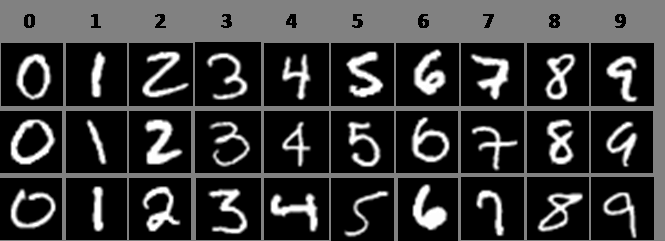
\includegraphics[scale=0.5]{pics/mnist_numbers.png}
	\caption{Ejemplo de input para entrenamientos y validaciones del KNN}
\end{figure}



\subsection{Entrenamiento del modelo}
Una vez finalizada la prueba de concepto, se comienza con el desarrollo del modelo, esto es, su proceso de creación, entrenamiento, validación, uso, etc. Para ello debemos subdividir esta sección en varias partes que, no obstante, están interrelacionadas, y por tanto pueden verse afectadas entre sí. A continuación se explican cada una de estas subtareas:

\subsubsection{Elección de librerías}
Existen ciertas librerías básicas de las que debemos partir. Para ello debemos realizar un estudio sobre las tecnologías y procesos que necesitaremos, qué funcionalidades vamos a desarrollar y de qué herramientas necesitaremos disponer. No obstante, a lo largo del desarrollo podremos ir necesitando librerías adicionales con las que no hayamos contado en primer lugar que habrá que tener en cuenta a la hora de documentar el proyecto.

En nuestro caso, se contempla inicialmente la posibilidad de utilizar PyTorch, una librería de IA bastante conocida y con amplia trayectoria, pero tras navegar a través de la documentación e informarse a través de diversas fuentes, se decide finalmente utilizar la librería de Tensorflow, debido a, entre otros motivos, una mayor facilidad de uso de su API, una documentación más extensa y explicativa, y mayor uso entre los desarrolladores actuales de IAs, lo que se traduce en mayor contenido e información respecto a los diversos problemas y opciones con las que nos enfrentamos durante el desarrollo.

Adicionalmente a la librería de Tensorflow, conocemos ciertas librerías que necesitaremos usar con seguridad a lo largo del desarrollo como PIL(Pillow) para manejo de imágenes, Matplotlib para generación de gráficos informativos, Keras como anexo a Tensorflow para el entrenamiento, Numpy para creación de matrices y otras colecciones con el poder computacional que ofrece C, y muy importante, Torch-directml para integrar entrenamientos de IA con gráficas de AMD a través de Direct-X12.

\subsubsection{Búsqueda del dataset}
Parte esencial de la creación de una IA, es utilizar un dataset adecuado, por lo que, a falta de capacidad y tiempo para generar uno propio, debemos buscar un dataset ya existente con los contenidos que necesitemos y, de si no cumpliese nuestras expectativas, adaptarlo a nuestras necesidades.

\begin{comment}
La elección del dataset se ve condicionada por la escasez de ellos. Esencialmente, podemos encontrar dos datasets distintos en todo internet, el primero siendo Kuzushiji-Kanji, que es el que finalmente se utilizara en este proyecto tras sopesar ventajas e inconvenientes, y ELTCDB. Aunque el primero es un dataset mucho más desfasado, incompleto y desbalanceado, viene muy convenientemente clasificado y listo para su uso, mientras que el segundo viene subdividido en diversos sets de caracteres, y con sus imágenes convertidas en formato binario anexadas unas detrás de otras, que habría que tratar correctamente bajo estrictas instrucciones proporcionadas por el AIST (National Institute of Advanced Industrial Science and Technology).

Debido a esto, aunque la eficacia de la IA se verá mermada por la integridad del dataset, la implementación del modelo puede hacerse casi de forma directa a través de la API de Keras.
Para compensar este desbalance del dataset, se crean dos programas .py. En el primero, generamos, en base a diferentes fuentes en japonés, una imagen acorde al formato de las imágenes de nuestro dataset de cada uno de los kanji pertenecientes al JLPT y la añadimos al dataset. En el segundo, recorreremos de nuevo nuestro dataset y eliminaremos de este todas las carpetas e imagenes de kanjis que se repitan menos de 5 veces, ya que consideramos que es un mínimo a partir del cual el hecho de que ese kanji exista en el modelo, produce más falsos resultados qué resultados correctos sin importar las correcciones que intentemos aplicar.
\end{comment}
La elección del dataset se ve condicionada por la escasez de éstos. Esencialmente, podemos encontrar dos datasets distintos en internet.

El primero es ELTCDB, que aunque a primera vista tiene una mejor calidad de datos, éstos vienen en un formato más incómodo para trabajar con él. Esencialmente, debes pedir permiso al AIST (National Institute of Advanced Industrial Science and Technology) para obtener acceso, y una vez concedido, todos los datos se encuentran en binario, subdivididos de forma irregular y bajo un estándar propio del AIST, quien te proporciona las instrucciones para decodificarlos correctamente.

Es por la complejidad en el proceso de obtener los datos en el formato que queremos, que se opta por la segunda opción: Kuzishiji-Kanji, que sí que viene en un formato conveniente para nuestro caso de uso. Como inconveniente de este dataset, cabe destacar que sus datos están ligeramente más desfasados, es algo más incompleto y está peor balanceado.

Sin embargo, aunque la eficacia de la IA se verá mermada por la integridad del dataset, elegimos este dataset, ya que la implementación del modelo puede hacerse casi de forma directa a través de la API de Keras.

Para compensar este desbalance del dataset, se crean tres scripts:
\begin{itemize}
	\item El primero genera, en base a diferentes fuentes en japonés, una imagen acorde al formato de las imágenes contenidas en nuestro dataset por cada kanji disponible para aumentar el número de muestras.
	\item El segundo se encarga de recorrer de nuevo el dataset, eliminando todas las carpetas e imágenes que contengan menos de diez muestras, el mínimo que consideramos para obtener un resultado consistente. Esto se hace teniendo en cuenta que el anterior script generará aproximadamente, 7 muestras por kanji.
	\item El tercero se encarga de normalizar el número de muestras. Lo ideal es que se entrene bajo un rango sin una gran discrepancia entre mayor y menor número de muestras. Para esto, en nuestro script se generan por data augmentation nuevas muestras en aquellos kanji por debajo de un umbral mínimo, y se eliminan muestras aleatorias en aquellos por encima de un umbral máximo. En nuestro caso, los umbrales se sitúan en 500 muestras máximo, y 80 mínimo.
\end{itemize}
Cabe destacar que los kanji en los que ocurre esto son, generalmente, muy poco comunes de ver, o que han caído en desuso.

\subsubsection{Diseño de la red neuronal}

Es importante realizar un estudio en profundidad de los diseños de redes neuronales recomendables para la funcionalidad que estamos buscando, y, posteriormente, analizar los resultados de la \hyperref[sec:terms]{\textit{validación}\tec} y realizar pruebas de los modelos generados utilizando esta red para poder ajustar sus parámetros de configuración acorde con el dataset que le vamos a proporcionar.\\

\noindent Antes de comenzar con explicaciones más técnicas, conviene conocer la siguiente terminología:
\begin{itemize}
	\item Capa: Una capa es el bloque más general dentro de un modelo de IA. Son contenedores que se encargan de recibir un dato de entrada, transformarlo a partir de determinadas operaciones matemáticas, y generar un dato de salida con el que informar a la siguiente (o generar un resultado final en el modelo). Las capas se dividen en \textit{input} y \textit{output layers}, siendo respectivamente la primera y la última capa del modelo, y \textit{hidden layers} siendo estas todas las que se encuentren entre las dos anteriores.
	\begin{figure}[!ht]
    	\centering
    	\label{fig:cnn}
    	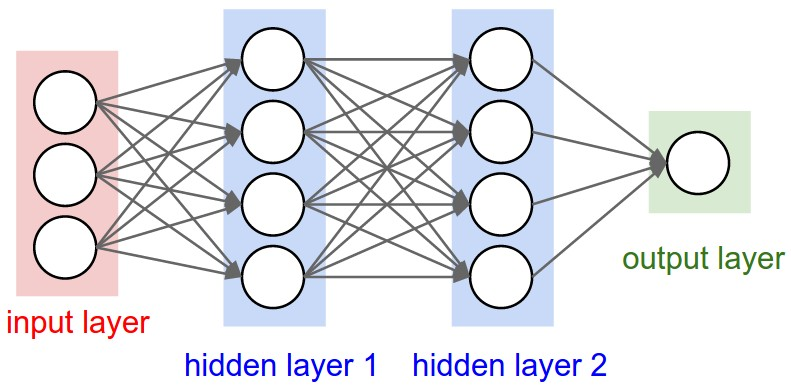
\includegraphics[scale=0.25]{pics/cnn.jpg}
    	\caption{Estructura de capas en una red neuronal.}
	\end{figure}
	\item Convolución: Se trata de una operación matemática que describe cómo fusionar dos partes de información, primero un dato de entrada (en nuestro caso concreto, el valor de cada píxel), y segundo el valor conjunto de todos los vecinos definidos por el kernel, para generar un mapa de características del dato inicial.
	\item Kernel: consiste en una pequeña matriz que itera sobre los datos de entrada, realizando determinadas operaciones entre el elemento seleccionado y los elementos de su alrededor y calculando un nuevo resultado para el elemento original.
	\begin{figure}[!ht]
    	\centering
    	\label{fig:conv}
    	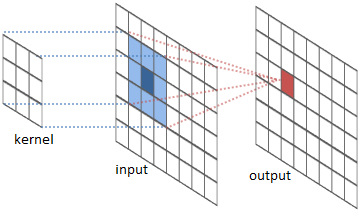
\includegraphics[scale=0.5]{pics/convolution.png}
    	\caption{Proceso de convolución de una imagen}
	\end{figure}
	\item Neurona: Al nivel más conceptual, una neurona es una función que opera sobre los datos de entrada ($x_n$), aplicándole unos pesos ($w_n$), y dando como resultado una salida ($y$) que puede ser procesada por una función de activación. Generalmente, cada una de estas unidades, se encuentra conectada en ambos sentidos a varias neuronas. Estas unidades pueden seguir diferentes patrones de conexión entre ellas o ser usadas en conjunto con múltiples funciones de activación.
	\item Peso: Son valores numéricos que se asocian a las conexiones entre las neuronas de diferentes capas. Estos se inicializan de forma aleatoria con la primera iteración del entrenamiento, y a partir de una serie de ecuaciones, son ajustados para las siguientes iteraciones acorde a los resultados obtenidos.
    	\begin{figure}[!ht]
    	\centering
    	\label{fig:perceptron}
    	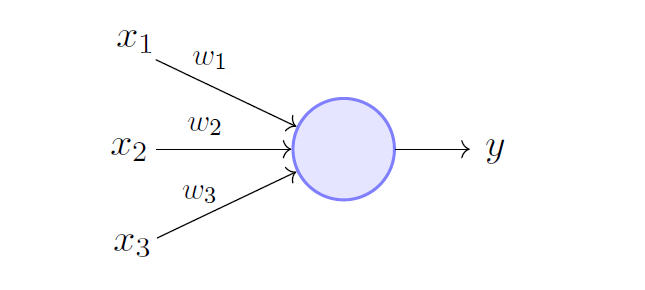
\includegraphics[scale=0.4]{pics/perceptron.png}
    	\caption{Representación del funcionamiento de una neurona}
	\end{figure}
	\item Activación: Las funciones de activación son operaciones matemáticas que se encargan de  transmitir la información generada por la neurona a las neuronas de la siguiente capa. La función de activación puede ser de muchos tipos según el resultado que se pretenda obtener. Algunos de estos tipos son Sigmoid (transformar los valores introducidos a una escala 0-1), Softmax (transformar el sumatorio de todas las salidas a 1) y que se utilizará en otros puntos relevantes del proyecto, o ReLU, como utilizamos en este caso (transformar los valores de entrada anulando los negativos y dejando los positivos sin modificar). En términos generales, se buscan funciones cuyas derivadas sean simples para minimizar al máximo el coste computacional del entrenamiento.

\end{itemize}

Vistos los términos más comunes que utilizaremos en nuestra explicación, los detalles específicos para nuestro proyecto se describen a continuación.

Se ha optado por un diseño de red convolucional (explicado más adelante) que sigue un patrón bastante extendido y recomendado para IAs cuyo objetivo es \textit{Optical Character Recognition} (\hyperref[sec:terms]{\textit{OCR}\tec}), como es nuestro caso.

En los párrafos a continuación, se procede a profundizar de forma más técnica este diseño, no obstante cabe destacar que no se ofrecen una gran cantidad de detalles con respecto a las propiedades de las herramientas que utilizamos, ya que son de una gran complejidad y se salen del objetivo de este documento.\\

Nuestra red neuronal está compuesta por dos bloques principales. Un primer bloque compuesto por capas de Convolución y Pooling que se encargarán de extraer información de las imágenes, y un segundo bloque compuesto por capas Densas.

Previo a las capas definidas a continuación, se aplican dos transformaciones extra, una de redimensionado, y una de reescalado, que transformarán los datos introducidos al modelo al tamaño y formato de datos requeridos por la capa inicial.

Las capas convolucionales se encargan de extraer la información relevante de la imagen a través de la iteración de un kernel por cada píxel de la imagen. Esto dará como resultado una imagen del mismo tamaño que la original donde cada píxel tendrá la información relevante sobre aquellos a su alrededor.

Las capas de MaxPooling2D, al igual que las Convolucionales, iteran un kernel por cada pixel de la imagen, pero al contrario que estas últimas, su objetivo es reducir el tamaño total de la imagen descartando los resultados menos relevantes, ayudando al modelo a  centrarse en las características de mayor importancia y reduciendo el tiempo de procesamiento.

A continuación de este grupo de capas, interviene una capa de Dropout, que fuerza al modelo a ignorar cierta cantidad de neuronas que se eligen de forma aleatoria en cada iteración del entrenamiento, de forma que se incentiva a la red a buscar caminos alternativos para la resolución del problema planteado. Esto previene que el algoritmo genere una dependencia a ciertas neuronas, reduciendo el \hyperref[sec:terms]{\textit{overfitting}\tec} y mejorando la capacidad de respuesta a nuevos datos.

\begin{figure}[!ht]
	\centering
	\label{fig:model}
	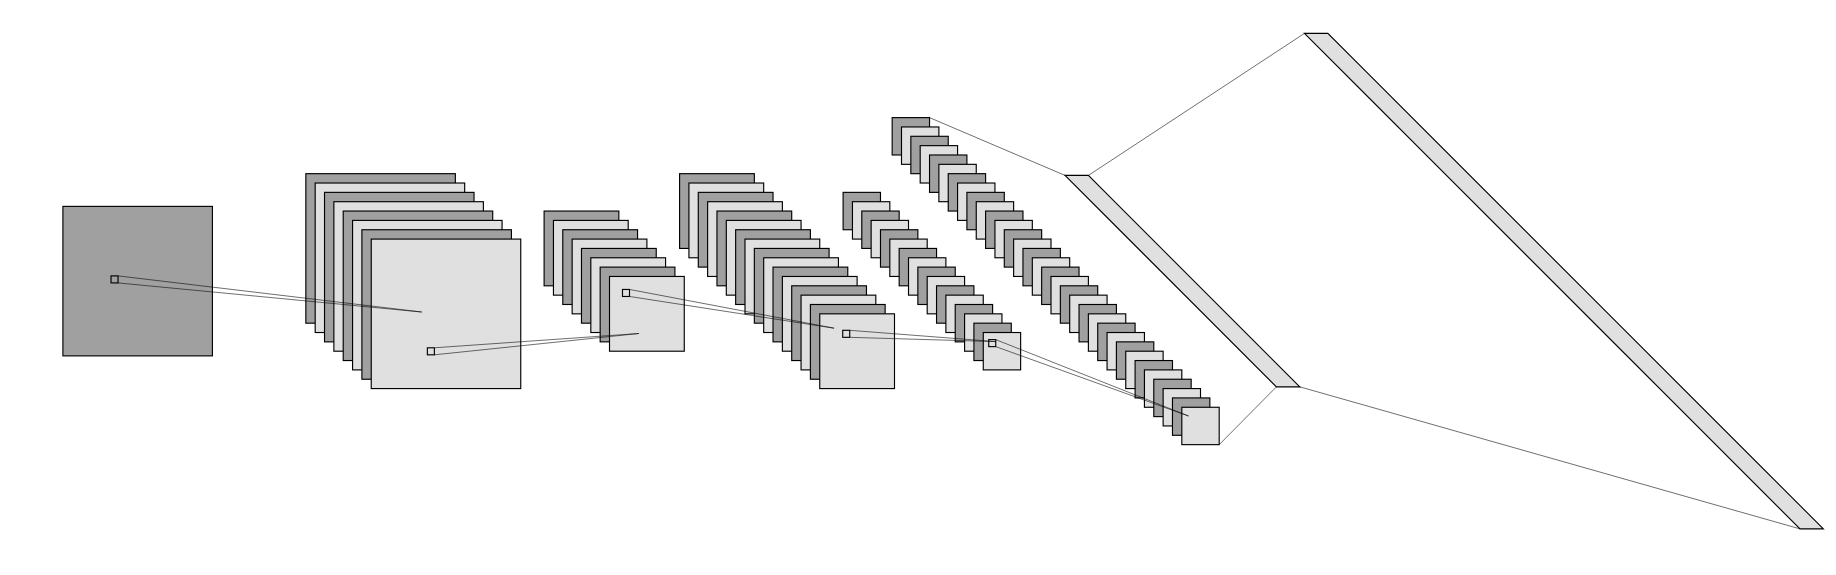
\includegraphics[scale=0.3]{pics/LeNetStyle.png}
	\caption{Representación LeNet de nuestro modelo}
\end{figure}

A través de una capa Flatten, simplemente transformamos los datos que hemos obtenido con las funciones anteriores en una secuencia lineal de forma que sea más simple para el algoritmo conectar los datos y entender el conjunto global de la imagen original en las siguientes capas del modelo.

Llegando al final del modelo, disponemos dos capas densas, intercaladas por otra capa Dropout. Las capas densas son aquellas donde el modelo pasa de analizar los datos a clasificarlos, para en la última capa generar un resultado final. En estas capas, cada neurona de la capa actual, está conectada a cada una de las neuronas de la capa anterior, y estas conexiones llevan asociadas un peso ajustado durante el entrenamiento. Son capas particularmente útiles en el reconocimiento de patrones. A las neuronas de estas capas también se les aplica una función de activación ReLU, que permite a la red aprender relaciones complejas entre los datos. La salida de datos tras pasar por este modelo viene directamente de la última capa densa, cuyo número de neuronas es igual al número de kanji disponibles en nuestro dataset. El valor de salida de cada una de las neuronas de la última capa, representará la probabilidad de que el kanji asociado a dicha neurona sea el mismo que el del dato de entrada.

También es importante remarcar que lo anterior es una explicación general del diseño y funcionamiento del modelo, realizado con una librería de alto nivel. El funcionamiento de esta NN y las funciones que lo componen es mucho más compleja y técnica de lo que se pretende explicar en esta documentación. Toda información al respecto puede obtenerse en la documentación oficial de Tensorflow.\\

\noindent\begin{minipage}{\textwidth}
\begin{lstlisting}[language=python]
model = Sequential([
	tf.keras.Sequential([
    	layers.Resizing(64, 64),
    	layers.Rescaling(1./255)
	]),
	layers.Conv2D(16, 3, padding='same', activation='relu'),
	layers.MaxPooling2D(),
	layers.Conv2D(32, 3, padding='same', activation='relu'),
	layers.MaxPooling2D(),
	layers.Conv2D(64, 3, padding='same', activation='relu'),
	layers.MaxPooling2D(),
	layers.Dropout(0.2),
	layers.Flatten(),
	layers.Dense(128, activation='relu'),
	layers.Dropout(0.2),
	layers.Dense(len(labels), name='outputs')
])
\end{lstlisting}
\end{minipage}\\\\\\


\subsubsection{Declaración del modelo}

\noindent\textbf{Terminología}
\begin{itemize}
	\item Batch: Se trata de un parámetro que se encarga de determinar el número de datos que se cargarán en memoria por cada iteración de la época actual del entrenamiento. Cuanto menor sea este número, más ruido se genera en el entrenamiento, pero mucho menor serán los recursos utilizados.
	\item Época: Se trata de un ciclo completo a través de todo el conjunto de datos de entrenamiento. El número de épocas indica la cantidad de iteraciones que el algoritmo de aprendizaje completará a lo largo de un proceso de entrenamiento.
	\item Función de pérdida: Es la función que se encarga de medir como de precisas son las predicciones que realice nuestro modelo con respecto a los resultados verídicos. El objetivo es conseguir que su resultado sea lo menor posible, es decir, que el ratio de error sea lo más pequeño posible. Aunque existen múltiples funciones de pérdida como Hinge Loss (clasificación binaria) o Mean Absolute Error (error promedio en tareas simples de regresión), en este caso se ha utilizado Categorical Cross-entropy, diseñada para tareas de clasificación multiclase, en la que se analizan las diferencias entre las probabilidades de la predicción y el valor real.
	\item Optimizador: Se trata de un algoritmo que se encarga de ajustar ciertos parámetros internos del modelo durante su entrenamiento, buscando minimizar el ratio de error, optimizando los pesos en base a los resultados de la función de pérdida aplicada al modelo. Existen numerosos algoritmos de optimización, y su elección dependerá de diversos factores como la velocidad de convergencia que queramos obtener, como de eficiente en términos de memoria queramos que sea, o los tipos de datos de entrada, entre otros. Algunos de los más utilizados son SGD(-Stochastic Gradient Descent-, que optimiza en base al gradiente general del modelo), RMSProp(-Root Mean Scope Propagation-, que optimiza en base al gradiente medio de los resultados más recientes), Momentum(que toma como base SGD, pero teniendo en cuenta también la media global en lugar de los resultados individuales), Adam(-Adapting Moment Estimation- que ajusta individualmente los parámetros combinando los algoritmos de RMSProp y Momentum)...
	\item Gradiente: Es un vector calculado en base a las derivadas parciales de nuestra función de pérdida y nuestro ratio de aprendizaje. Simplificando, es una guía que utiliza nuestro algoritmo para modificar sus pesos de forma dinámica y generar mejores resultados, es decir, si nuestro objetivo es llegar al punto 0 en una curva descendente de errores, el gradiente sería la verticalidad de la pendiente de la curva.

\begin{figure}[!ht]
	\centering
	\label{fig:gradex}
	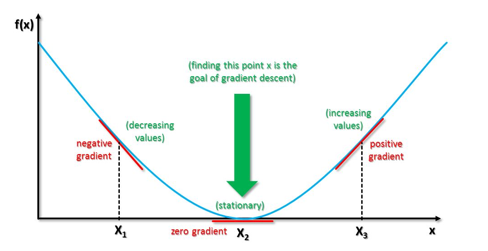
\includegraphics[width=0.7\textwidth]{pics/gradexp.png}
\end{figure}
    
	\item Momentum: Aunque se ha mencionado anteriormente como un optimizador per se, es un concepto importante en el uso de optimizadores para IA, que puede usarse como parámetro en varios de ellos. En nuestro caso, utilizando el algoritmo Adam, no es necesario, ya que es un algoritmo adaptativo, pero en muchos otros optimizadores es necesario definir esta variable, que se encarga de superar el falso mínimo con el que el optimizador va a toparse en su entrenamiento. La función de pérdida no siempre genera una derivada con una curva regular, en muchas ocasiones, la curva tendrá numerosas subidas y bajadas. Es para conseguir ignorar el mínimo local que existe este parámetro, definiendo un rango de gradiente ascendente a ignorar, que haga que el entrenamiento siga adelante a pesar de haber alcanzado un mínimo aparente.
\end{itemize}
\begin{figure}[!ht]
	\centering
	\label{fig:grad}
	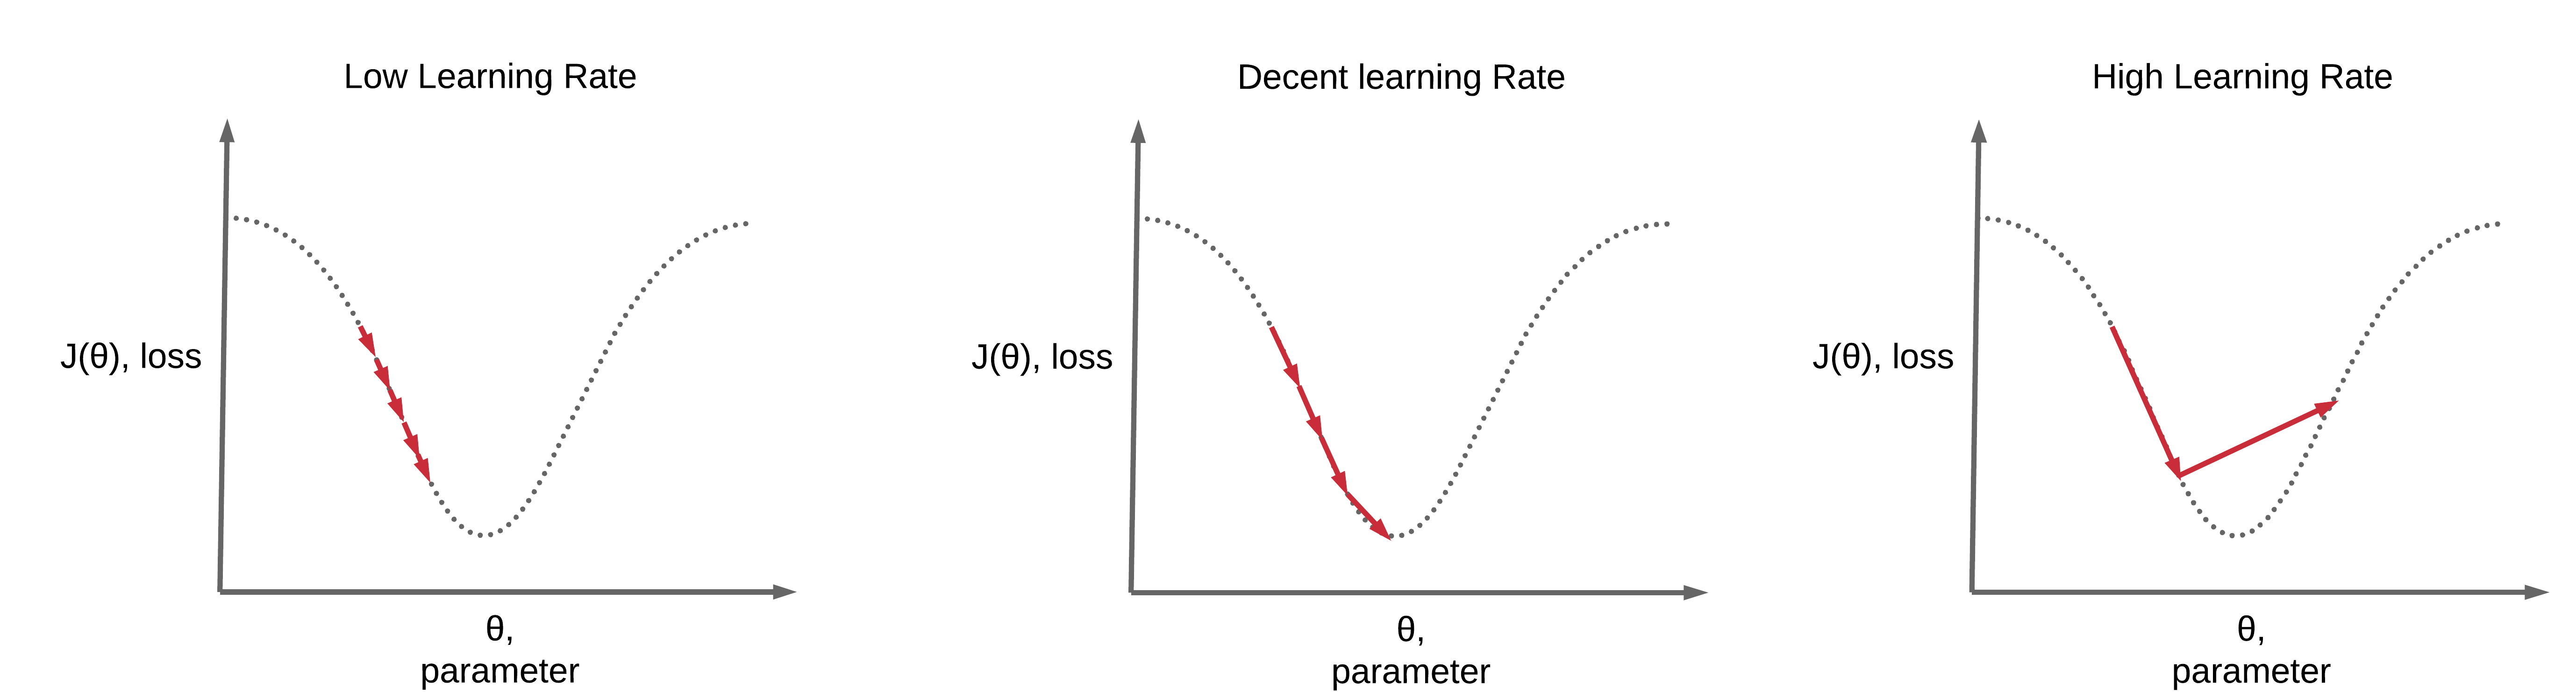
\includegraphics[width=1\textwidth]{pics/gradient.png}
\end{figure}

Dado el diseño de la red neuronal definido en el punto anterior, comenzamos con la declaración del modelo con vistas a su entrenamiento, guardado, validación y posterior uso.

%TODO: Reescribir
Es importante destacar que el entrenamiento de una IA tiene una gran parte de ensayo-error, por lo que en el código que veremos a continuación, aunque los parámetros son los utilizados en el entrenamiento final del modelo, para llegar a ellos han sido necesarios muchos intentos y modificar muchas variables junto con las comprobaciones posteriores pertinentes hasta llegar a ellos.

La declaración del modelo y otros parámetros necesarios, se definen a través de la API de Tensorflow junto con Keras, que pone a nuestra disposición numerosas utilidades de las cuales podemos informarnos a través de su documentación oficial. El código se muestra a continuación:

\noindent\begin{minipage}{\textwidth}
\begin{lstlisting}[language=python]
dataset_dir = pathlib.Path('instalation/data/Kanji_Images')  

batch_size = 32  
source_height = 64  
source_width = 64  

training_dataset = tf.keras.utils.image_dataset_from_directory(
	dataset_dir,  
	validation_split=0.2,  
	subset='training',  
	seed=39,  
	image_size=(source_height, source_width),  
	batch_size=batch_size)  

validation_dataset = tf.keras.utils.image_dataset_from_directory(
	dataset_dir,
	validation_split=0.2,
	subset='validation',
	seed=39,
	image_size=(source_height, source_width),
	batch_size=batch_size)
    
optimizer_model = keras.optimizers.Adam(learning_rate=0.0005)
loss_model = tf.keras.losses.SparseCategoricalCrossentropy(from_logits=True)
model.compile(optimizer=optimizer_model,
          	loss=loss_model,
          	metrics=['accuracy'])
epochs = 50
training = model.fit(training_dataset,
                 	validation_data=validation_dataset,
                 	epochs=epochs)
model.save('trainings/fullmodel2.keras')
\end{lstlisting}
\end{minipage}\\

En primer lugar, nos encargamos de crear las variables que contendrán el directorio de nuestro dataset, el tamaño del batch, y el alto y ancho de las imágenes de nuestro dataset.

A continuación, definimos los dataset de entrenamiento y validación a través de una de las herramientas ofrecidas por Keras, a las que le pasaremos el directorio, el porcentaje de separación aleatoria entre dataset de entrenamiento y validación, el nombre del subset, una semilla de aleatoriedad para evitar que la IA se acostumbre a determinados patrones, el tamaño de nuestras imágenes y el tamaño de nuestro batch.

Finalmente, inicializamos nuestras variables para el optimizador y nuestra función de pérdida. El optimizador utilizado para este caso ha sido Adam, ya que tras numerosas pruebas, el entrenamiento más correcto y eficiente en términos computacionales era este. Lo utilizamos, como podemos ver en el código, con un learning rate de 0.0005. Nuestra función de pérdida sera SparseCategoricalCrossentropy.

Con todas estas variables correctamente definidas, podemos realizar la compilación de nuestro modelo pasándole las variables que acabamos de crear, definir un número de épocas, y llamar a la función .fit(), que se encargará de hacer una iteración de entrenamiento por el número de épocas especificado. En nuestro caso, además, asignamos el valor devuelto por esta función a una variable que nos será útil más adelante en el código para consultar valores y generar gráficos de los resultados obtenidos en el entrenamiento.

Finalmente, utilizamos la función .save() de nuestro modelo para que se genere un archivo en cuyo interior se almacenan los pesos del modelo entrenado, que podremos cargar mas tarde para realizar las predicciones necesarias.\\


Todos estos términos tienen un fuerte componente matemático detrás, que se extiende al objetivo de este documento, por lo que las explicaciones plasmadas aquí únicamente pretenden clarificar al lector acerca de los términos utilizados y el papel que juegan en el desarrollo del proyecto.

Para más información respecto tanto al contexto matemático como a las diferentes definiciones y usos de las herramientas mencionadas en esta sección, pueden consultarse las fuentes que figuran en el anexo de información adicional externa:\\


\subsubsection{Validación}
Con cada época del entrenamiento, es convención en desarrollo de IA realizar una validación de este, para ver que progresa como es debido y los resultados avanzan en la dirección adecuada, hasta llegar a una validación con la que estemos satisfechos que nos indique que el modelo que hemos entrenado está listo para su uso. En este punto debemos desarrollar una herramienta que compruebe tanto con datos del dataset, como externos a él, que las predicciones que realiza de los datos que le pasamos son acertadas con suficiente certeza y el suficiente número de veces.

Es importante realizar un batch de validación porque entrenar una IA y validar con el mismo set de datos con la que la hemos entrenado no es recomendable; en primer lugar, no sabemos si es capaz de reconocer datos que le sean desconocidos, y en segundo lugar, las métricas que recibamos sobre la precisión y la tasa de acierto se verán afectadas precisamente por haberse entrenado con los mismos datos que intentamos predecir.

La idea detrás de este desarrollo es poder obtener información precisa sobre el rendimiento de nuestra IA, de forma que podamos ajustar sus parámetros en base a ensayo-error (práctica muy común en entrenamiento de IAs) hasta dar con unos ajustes cuyo rendimiento sea satisfactorio. Esto nos permitirá entrenar un número considerable de épocas, hasta que los resultados de la validación muestren un estancamiento del ratio acierto/error.

Cabe mencionar que es en este punto donde debemos dejar de entrenar la IA, ya que forzarla a continuar un número excesivo de épocas para conseguir mejoras marginales, puede generar el llamado \hyperref[sec:terms]{\textit{overfitting}\tec}, que causara un mayor número de falsos resultados a la hora de trabajar con datos ajenos al dataset original.


\subsection{Implementación}

En esencia, debemos encargarnos de que nuestra IA pueda ser utilizada accediendo a ella sin necesidad de ejecutar manualmente un script (como hacemos con nuestra validación), y que los datos que esta genera, puedan ser recibidos e interpretados por otras herramientas en lugar de ser impresos en una consola. Para ello, se distinguen dos puntos fundamentales que desarrollamos a continuación.

Para conocer en detalle el funcionamiento interno, casos de uso de la aplicación, etc. se incluyen varios diagramas UML disponibles en el \hyperref[sec:uml]{\textit{Anexo 2.}}

\subsubsection{Configuración de los métodos}
Siguiendo la documentación oficial de la librería que utilicemos, debemos definir los parámetros que la API desea recibir, el protocolo utilizado, la ruta donde desea recibirlos, y demás configuraciones necesarias para después poder consumir esa funcionalidad a través de protocolo HTTP, ya sea utilizando \hyperref[sec:terms]{\textit{Postman}\tec} o un navegador.

En este caso, tras todo el desarrollo de la IA, se hace una búsqueda sobre las librerías con las que podemos proceder a crear la API. Se decide utilizar las librerías de FastAPI y Uvicorn. La primera librería se encargará de permitirnos crear las funcionalidades que necesitemos para interactuar con nuestro código. La segunda se trata de una implementación para Python de un servidor web ASGI, lo que nos permitirá acceder a él a través de una red.

Una vez configurada la API y levantado el web service con uvicorn, comprobamos que todos estos métodos y la configuración del servicio funcionen correctamente, intentando realizar una request a través de Postman. Una vez consigamos que la respuesta HTTP devuelta sea satisfactoria, aunque no tengamos nuestro resultado, confirmaremos que la configuración de estos puntos es la correcta, y necesitará poca o ninguna configuración extra de aquí en adelante.

\subsubsection{Presentación del resultado}
Una vez desarrollada correctamente la configuración de la API, faltaría la parte del desarrollo en la que los datos que hemos enviado a nuestro servidor se procesan y recibamos una respuesta en el formato correcto con los datos que ha generado nuestra IA.

Será trabajo de otras herramientas utilizadas cómo procesar la información enviada por nuestra API, sin embargo el formato en el que esta envíe los datos debe ser algo legible y fácilmente procesable, por lo que nuestro resultado se configura para que devuelva un JSON formateado de forma específica para su posterior lectura.

\noindent\begin{minipage}{\textwidth}
\begin{lstlisting}[title=Formato del JSON de respuesta., numbers=none]
	{
  	"result": [
    	{
    	"character": "kanji1",
    	"certainty": "0.5"
    	},
[...]
    	{
    	"character": "kanji5",
    	"certainty": "0.04"
    	}
  	]
	}
\end{lstlisting}
\end{minipage}

\subsection{Alojamiento}
Uno de los objetivos de este proyecto es poder consumir la IA a través de un WebService expuesto a internet, por lo que uno de los pasos a seguir será configurar un servidor privado donde alojar la API y exponer sus funcionalidades a internet. Para realizar este punto, debemos seguir los siguientes pasos:

\subsubsection{Montaje e instalación del servidor}
Se plantea usar como servidor una torre de bajo presupuesto. En este ordenador se instalará la versión estable mas reciente de \hyperref[sec:terms]{\textit{Linux Debian}\tec}, sin ningún tipo de interfaz gráfica ni utilidades extras a las propias del Sistema Operativo a parte de Docker, para la creación de \hyperref[sec:terms]{\textit{containers}\tec}; Git, para descarga y manejo de repositorios; y NeoVim, un editor de texto de terminal para gestionar los archivos de configuración necesarios en el servidor

La instalación y configuración inicial se realiza de la forma habitual, y una vez configurada la red y el acceso por \hyperref[sec:terms]{\textit{SSH}\tec}, desconectamos todos los periféricos y utilizamos una conexión SSH para acceder a él sin necesidad de compartir o utilizar periféricos extra, conectándonos desde el mismo sistema desde el que realizamos nuestro desarrollo.

Esto es particularmente útil ya que quitamos del servidor cualquier tipo de software que pueda consumir sus recursos de forma innecesaria. En su lugar, trabajamos con el mismo equipo con el que desarrollamos y configuramos todas las características propias del código fuente, y a través de una consola de comandos, modificamos y configuramos aquello que necesitemos en nuestro servidor de forma remota.

\subsubsection{Networking}
Para que el sistema que instalamos en el punto anterior pueda realizar las funciones de servidor que necesitamos, tenemos que realizar diversos ajustes de \hyperref[sec:terms]{\textit{networking}\tec} que explicamos a continuación.\\

En primer lugar, debemos asegurarnos una \hyperref[sec:terms]{\textit{IP pública}\tec}. Para esto, se contacta con nuestro \hyperref[sec:terms]{\textit{ISP}\tec}, y se le solicita que se nos asigne una \hyperref[sec:terms]{\textit{IP dinámica}\tec} fuera del \hyperref[sec:terms]{\textit{CGNAT}\tec}.

Hecho esto, le asignamos a nuestro servidor una \hyperref[sec:terms]{\textit{IP estática}\tec} dentro de nuestra red local, y la asignamos a un \hyperref[sec:terms]{\textit{dominio}\tec} de tal forma que las conexiones del exterior siempre accedan a través de la misma dirección.

Legalmente, nuestro ISP tiene la obligación de proveernos una IP pública, sacándonos del CGNAT en el que nos tengan. Por suerte, O2 (Telefónica) únicamente asigna IPs públicas a sus clientes, por lo que durante este desarrollo no se ha necesitado llevar a cabo este trámite.

Técnicamente, también tienen la obligación de proveernos una IP estática, sin embargo, al contrario que una IP dinámica como mencionamos anteriormente, esto no se contempla de forma gratuita, sino que se trata de un servicio de pago.

Dado que para este proyecto ya disponemos de una IP pública, nos es suficiente para poder configurar el servidor acorde a nuestras necesidades. En primer lugar, se compra un dominio a través de Namecheap.com (otterleek.com). A continuación, nos registramos en NoIP.com, un servicio gratuito que se encarga de monitorizar nuestra IP y asignarle de forma dinámica un \hyperref[sec:terms]{\textit{DNS}\tec} desde el que poder conectarte.

En términos generales, la IP pública que nos proporciona nuestro ISP se mantiene hasta que nuestro router se reinicia o pierde su conexión. Si en algún momento el ISP cambia nuestra IP, NoIP.com lo detecta, y apunta el dominio que hemos solicitado a nuestra nueva IP. NoIP ofrece este servicio de forma gratuita con la condición de confirmar una vez al mes que continuamos utilizando sus servicios.

Solucionado el problema de que podamos acceder a nuestra IP en cualquier momento que queramos independientemente de si ha cambiado o no, quedaría reasignar nuestro dominio al que hemos adquirido. Para ello la propia página de Namecheap tiene unas opciones de configuración DNS con las que podremos realizar estos cambios. Para nuestra IA crearemos un subdominio al que podremos enviar una petición HTTP (kanji.otterleek.com) que apuntaremos al DNS facilitado por NoIP.

Con esta configuración ya tendríamos el networking listo para poder configurar un container a través del que podremos hacer consultas sobre nuestro web service.

\subsubsection{Dockerización}
Por último, dentro de nuestro servidor, para que pueda convivir con más aplicaciones y herramientas, instalaremos nuestra API en un container de Docker y le asignaremos el puerto que deseemos, asegurándonos de que todo está correctamente expuesto a internet y que el container es capaz de mantenerse activo sin mantenimientos adicionales.

\noindent El proceso para esto es bastante simple. En nuestro directorio root del servidor, introducimos los comandos

\noindent\begin{minipage}{\textwidth}
\begin{lstlisting}[numbers=none]
mkdir -p Docker/Kanji-AI && cd $_
nvim Dockerfile
\end{lstlisting}
\end{minipage}
Esto creará un directorio donde almacenaremos toda la configuración de nuestro container y un archivo Dockerfile donde definiremos los parámetros de instalación e inicialización del container:

\noindent\begin{minipage}{\textwidth}
\begin{lstlisting}[numbers=none]
FROM python:3.8
WORKDIR /code
COPY ./requirements.txt /code/requirements.txt
RUN pip install --no-cache-dir --upgrade -r /code/requirements.txt
COPY ./app /code/app
CMD ["uvicorn", "app.main:app", "--proxy-headers", "--host", "0.0.0.0", "--port", "39000"]
\end{lstlisting}
\end{minipage}
Para que el proyecto funcione correctamente deberá instalar una serie de librerías que le pasamos en un archivo de texto llamado \textit{requirements.txt} como puede verse en el fichero anterior, que debemos crear con el siguiente contenido:

\noindent\begin{minipage}{\textwidth}
\begin{lstlisting}[numbers=none]
fastapi>=0.68.0
pydantic>=1.8.0
uvicorn>=0.15.0
numpy
tensorflow
pillow
python-multipart
matplotlib
\end{lstlisting}
\end{minipage}

Este proceso creará una instalación del container con las dependencias necesarias, sin embargo, necesitamos configurarlo correctamente para que al levantarse, se conecte correctamente con los puertos indicados, en la network adecuada, y a través del protocolo HTTPS.

Para esto debemos crear un \textit{docker-compose.yml}, aunque antes debemos realizar una correcta instalación y configuración de Traefik, un \hyperref[sec:terms]{\textit{reverse-proxy}\tec} y \hyperref[sec:terms]{\textit{load-balancer}\tec} integrado nativamente con Docker para permitirnos exponer a internet servicios desde nuestros containers. Como la configuración de Traefik es compleja y extensa, y va más allá del objetivo de esta documentación, estará disponible una breve explicación en el \hyperref[sec:Traefik]{\textit{Anexo 3}} sobre configuración de Traefik.

Una vez realicemos la correcta instalación y configuración de Traefik, podremos crear el fichero mencionado anteriormente con el siguiente contenido:

\noindent\begin{minipage}{\textwidth}
\begin{lstlisting}[numbers=none]
name: kanjiAI
services:
	kanjiAI:
    	build: .
    	image: kanji-AI
    	container_name: kanji-AI
    	working_dir: /code/app
    	command: "uvicorn main:app --host 0.0.0.0 --port 39000 --reload"
    	ports:
        	- "39000:39000"
    	volumes:
        	- .app:/code/app
    	restart: "unless-stopped"
    	networks:
        	- traefik-global-proxy
    	labels:
        	- "traefik.enable=true"
        	- "traefik.http.routers.ai.rule=Host(`kanji.otterleek.com`)"
        	- "traefik.http.routers.ai.tls.certresolver=letsencrypt"
        	- "traefik.http.routers.ai.entrypoints=https"
        	- "traefik.http.services.ai-service.loadbalancer.server.port=39000"
networks:
	traefik-global-proxy:
    	external: true
   	 
\end{lstlisting}
\end{minipage}

Tras realizar esta configuración, debemos abrir el puerto 39000 TPC en nuestro router. Podemos hacer esto accediendo a él a través de nuestra puerta de enlace y utilizando el software que los propios router implementan.

Por último, debemos incluir nuestro desarrollo en una carpeta llamada \textit{app/} (como puede verse en los archivos de configuración) dentro de nuestra carpeta de configuraciones del container, y levantar el container en modo detached para que el proceso del container no inutilice nuestra consola.

\noindent\begin{minipage}{\textwidth}
\begin{lstlisting}[numbers=none]
docker compose up -d
\end{lstlisting}
\end{minipage}
Nuestra IA estaría en este punto lista para utilizarse a través de internet, y podemos comprobar su correcto funcionamiento haciendo una petición HTTP \hyperref[sec:terms]{\textit{multipart}\tec} al dominio mencionado anteriormente (https://kanji.otterleek.com) con una imagen adjunta. La imagen llegará entonces a nuestro WebService y nuestro desarrollo realizará una predicción de los cinco kanjis más posibles en esa imagen, devolviéndonos una respuesta HTTP en el formato JSON mencionado previamente en esta misma sección.

\subsection{Creación de la interfaz}

Respecto a la creación de la interfaz, simplemente distinguiremos dos desarrollos, el diseño de la interfaz incluyendo sus funcionalidades, disposición y la interacción entre sus ventanas por un lado, y el desarrollo para contactar con el web service y procesar sus respuestas por otro.

\subsubsection{Frontend}
La intención original es que la app sea extremadamente simple, disponiendo de dos funcionalidades básicas, capturar una imagen (únicamente para dispositivos con cámara), y cargar una imagen desde la memoria del dispositivo.

Una vez cargada, mostrará la imagen a enviar para asegurarnos de que se ve correctamente y el caracter está correctamente acotado en la imagen para solicitar su predicción, junto con dos botones, uno para eliminar la imagen seleccionada y repetir el proceso, y otro para contactar con el web service, que una vez pulsada, esperará la respuesta de éste, y nos llevará a una ventana donde se muestre la predicción junto con el botón de salida.

\begin{comment}
Para todo este proceso, tanto la explicación del código como de la ejecución son demasiado específicos y aportan demasiado poco a la memoria del proyecto, por lo que considero que lo único a explicar en este apartado es que hemos decidido utilizar Flutter, un framework de Dart para diseno de aplicaciones multiplataforma que permite reutilizar nuestro código con mínimas modificaciones para crear aplicaciones en diferentes sistemas y plataformas.
\end{comment}
Para todo este desarrollo hemos utilizado Flutter, un framework basado en el lenguaje Dart enfocado en el desarrollo de aplicaciones multiplataforma que permite reutilizar nuestro código con las modificaciones mínimas para crear versiones para los dispositivos más utilizados hoy en día.

El desarrollo de la interfaz es una simple estructura de componentes, por lo que no considero necesario entrar en detalle sobre el código como tal, que estará disponible en el repositorio. Para cualquier información relativa a esta parte del desarrollo, puede consultarse la documentación oficial de Flutter.

\subsubsection{Back end}
Respecto a la funcionalidad que se desarrolle por debajo de la interfaz, nos centraremos casi de forma exclusiva en poder enviar la imagen al web service correctamente, y ser capaces de recibir y procesar su respuesta para mostrarla por pantalla.

Hay diversas utilidades para hacer que el dispositivo cargue una imagen de la galería o acceda a la cámara para capturar una imagen, por lo que no nos vamos a detener en la explicación de esto, sin embargo, la parte compleja de este desarrollo consiste en realizar satisfactoriamente una petición HTTP multipart que nos permita enviar la imagen a nuestro WebService, y recibir y formatear su respuesta correctamente.

Esta parte del desarrollo se sustenta sobre dos fragmentos de código que explico a continuación.

Flutter implementa nativamente el envío de peticiones HTTP multipart, por lo que hemos utilizado la siguiente función para solicitar una predicción a nuestra IA:

\noindent\begin{minipage}{\textwidth}
\begin{lstlisting}[language=java]
Future<Prediction> requestPredictionAPI(File kanji, BuildContext context) async{
	final request = http.MultipartRequest('POST', Uri.parse('https://kanji.otterleek.com/'));
	request.files.add(await http.MultipartFile.fromPath('file', path!));
	final response = await request.send();
	if (response.statusCode==200){
    	String b = (await http.Response.fromStream(response)).body;
    	return Prediction.fromJson(jsonDecode(b));
	}
	else{
    	Navigator.of(context).push(MaterialPageRoute(builder: (context) => Unavailable()));
    	throw Exception('Kanji AI Predict WebService is unavailable');
	}
}
\end{lstlisting}
\end{minipage}\\

Donde Prediction es una clase que recoge la respuesta HTTP y la transforma en consecuencia para poder acceder a los datos de respuesta desde el código más adelante:

\noindent\begin{minipage}{\textwidth}
\begin{lstlisting}[language=java]
class Prediction{
	final List<Content> content;
	Prediction({
    	required this.content,
	});
	factory Prediction.fromJson(Map<String, dynamic> json) => Prediction(
    	content: List<Content>.from(json['result'].map((x) => Content.fromJson(x))));
	Map<String, dynamic> toJson() => {
    	"result": List<dynamic>.from(content.map((e) => e.toJson()))
  };
}

class Content {
	final String character;
	final double certainty;
	Content({
    	required this.character,
    	required this.certainty
	});
	factory Content.fromJson(Map<String, dynamic> json) => Content(character: json['character'], certainty: json['confidence']);
 
	Map<String, dynamic> toJson() => {
    	"character": character,
    	"certainty": certainty
	};
}
\end{lstlisting}
\end{minipage}




%%%%%%%%%%%%%%%%%%%% PUNTOS DE MEJORA %%%%%%%%%%%%%%%%%%%%%%%
\newpage

\section{Puntos a mejorar}
\label{sec:Improvements}

Aunque la realización de este proyecto es satisfactoria, debido a la falta de tiempo, capacidades, u otras variables, algunos aspectos de este proyecto tienen una amplia capacidad de mejora. En este punto trataremos brevemente futuras mejoras a desarrollar para nuevas versiones. Mencionar antes de nada, que el objetivo de este apartado no es presentar aspectos con los que ampliar la funcionalidad de la aplicación, sino para elaborar puntos de mejora en el rendimiento, la facilidad de uso, etc. considerables que no se han podido aplicar por diversas circunstancias.

\begin{itemize}
	\item \textbf{Utilizar \hyperref[sec:terms]{\textit{data augmentation}\tec}}: El uso de data augmentation puede mejorar mucho la capacidad predictiva de la IA en casi cualquier escenario, sin embargo, no se ha implementado porque para esto se requiere de un poder computacional y un tiempo de entrenamiento muy elevado.
	\item \textbf{Implementar distinción de kanjis}: Se podría implementar un algoritmo capaz de analizar la imagen e identificar kanji que pueda haber en ella, y generar un encuadre correcto en torno a la figura para el posterior análisis por parte de nuestra IA. Esto haría que la experiencia de usuario y los casos de uso mejorasen sustancialmente, sin embargo no se ha considerado su implementación tanto por el factor de tiempo como por el de dificultad.
	\begin{comment}
	Realizar segmentación en las imágenes haría que no fuese necesario cuadrar en el centro de la imagen un kanji y asegurarnos de que está lo más aislado posible de otros elementos. Esta condición es una de las que más entorpecen el funcionamiento y la experiencia de esta herramienta, por lo que es un punto a considerar muy importante, sin embargo no se ha implementado por la dificultad que supondría la generación del algoritmo necesario para reconocer la parte necesaria y reformatear la imagen en consecuencia.
	\end{comment}
	\item \textbf{Mejorar el procesado de imágenes}: La IA es propensa a fallos cuando las fotografías se realizan en escenarios de poca luz debido al poco rango dinámico de los dispositivos, la cantidad de ruido, y el poco contraste presente en las imágenes tomadas en estas circunstancias. Un procesamiento de la imagen más exhaustivo, que analice la cantidad de luz, el contraste de la escena, y sea capaz de proveer un kanji en el mayor número de condiciones desfavorables posibles es un aspecto importante a tener en cuenta.
	\item \textbf{Interfaz más profesional}: El mayor peso de este proyecto recae sobre todo el proceso de creación de la IA y la comunicación con ella, por lo que la interfaz de usuario es excesivamente simple y con muy pocas funcionalidades. Es necesario considerar cambiar este diseño para sus futuras versiones y a ser posible añadir alguna funcionalidad extra para la comodidad del propio usuario.
	\item \textbf{Crear un instalador}: Se contempla como uno de los futuros desarrollos, una forma de crear un instalador de esta IA de forma que se aloje localmente en un dispositivo y podamos acceder a ella a través de una conexión local sin necesidad de acceder a internet. También facilitará todo el proceso de entrenamiento, que actualmente se lleva a cabo lanzando los scripts manualmente en el orden indicado en el archivo README. Este documento está disponible en la página principal del repositorio y en el \hyperref[sec:DevGuide]{\textit{Anexo 3.}}
\end{itemize}

%%%%%%%%%%%%%%%%%%%% RECURSOS %%%%%%%%%%%%%%%%%%%%%%%


\newpage
\section{Recursos}
\label{sec:Resources}

\noindent El detalle de todos los recursos utilizados en este proyecto consiste en:
\subsection{Recursos humanos}
\label{sec:HumanRes}

Los recursos humanos son virtualmente inexistentes. El proyecto se desarrolla de forma unipersonal, gestionando mi tiempo y mis recursos para la conclusión de los objetivos marcados en éste.

Únicamente cabe destacar la ayuda puntual de compañeros de clase, de profesión, y personal docente del centro que se verá reflejada en el anexo de agradecimientos.

\subsection{Hardware}
\begin{itemize}
	\item Un smartphone donde realizar pruebas de la aplicación móvil
	\item Un ordenador donde se desarrollará el proyecto junto con sus periféricos compuesto por:
	\begin{itemize}
    	\item CPU AMD Ryzen5 5600
    	\item GPU AMD Radeon 6600
    	\item RAM Viper 32Gb DDR4
    	\item SSD M.2 500Gb Crucial
    	\item Otros componentes (PSU, Fuente de Alimentación, Caja...)
    	\item Teclado Logitech MX Keys
    	\item Raton Logitech MX Master M3s
    	\item Monitores AOC 24G2U (x2)
	\end{itemize}
	\item Un servidor compuesto por:
	\begin{itemize}
    	\item CPU Intel i3 2120
    	\item RAM Kingston 6Gb DDR
    	\item SSD SATA3 Kingston 160Gb
    	\item Otros componentes (PSU, Fuente de Alimentación, Caja...)
	\end{itemize}
	\item Diversos cables de conexión, corriente, etc. (Ethernet, HDMI, DP, USB-C...)
\end{itemize}

\subsection{Software y Servicios}
\begin{itemize}
	\item Un dominio ("otterleek.com")
	\item Una conexión a Internet (O2)
	\item Licencias:
	\begin{itemize}
    	\item PyCharm Community Edition
    	\item Debian 12.2
    	\item Docker
    	\item Visual Studio Code
    	\item Postman
    	\item Overleaf
	\end{itemize}
	\item Diversas librerías de terceros (Tensorflow, Keras, Pillow...) que han sido mencionadas a lo largo del proyecto
\end{itemize}
\newpage

\subsection{Presupuesto}

El total del presupuesto incluye los 5 meses de desarrollo de la aplicación, y un solo año de dominio, sin embargo con futuros desarrollos, debido al pago de estos servicios, puede verse incrementado.

Algunos componentes son piezas genéricas de fabricantes que no están disponibles al público para su compra, por lo que ha sido todo agrupado bajo un mismo nombre genérico, y su precio se ha calculado en base a precios de componentes de características similares, al igual que con los cables utilizados, muchos proveídos por los propios fabricantes de los componentes. Estos elementos son: caja, placa base y fuente de alimentación del servidor, pilas CMOS, pasta térmica, cables SATA, cables HDMI, cables DisplayPort, cables USB y USB-C y cables de alimentación.\\
    
\begin{center}
    
\begin{tabularx}{\linewidth}{
| >{\raggedright\arraybackslash}X
 >{\raggedleft\arraybackslash}X
 >{\raggedleft\arraybackslash}X |
}
\toprule
Detalle                 	&	Cantidad       	&  Precio\\
\midrule

Asus Prime b550-Plus    	&	x1 ud.         	    &  109.99\euro\\
AMD Ryzen5 5600         	&	x1 ud.         	    &  137.52\euro\\
Intel i3 2120           	&	x1 ud.         	    &  32.46\euro\\
Xilence XC032           	&	x1 ud.         	    &  16.01\euro\\
XFX Speedster SWFT 210  	&	x1 ud.         	    &  229.90\euro\\
Viper 16Gb DDR4 3600mHz 	&	x2 ud.         	    &  36.59\euro\\
Kingston 4Gb DDR3 1333mHz   &	x1 ud.            	&  22.14\euro\\
Kingston 2Gb DDR3 1333mHz   &	x1 ud.            	&  17.24\euro\\
M.2 Crucial 500Gb       	&	x1 ud.         	    &  40.99\euro\\
SATA3 Kingston 160Gb    	&	x1 ud.         	    &  21.80\euro\\
SeaSonic Core GM 500W   	&	x1 ud.         	    &  86.99\euro\\
Lian Li Mesh 205        	&	x1 ud.         	    &  61.72\euro\\
AOC 24G2U               	&	x2 ud.         	    &  255.10\euro\\
Logitech MX Keys        	&	x1 ud.         	    &  89.99\euro\\
Logitech MX Master M3    	&	x1 ud.        	    &  91.41\euro\\
Xiaomi Redmi Note 12 Pro 5G &	x1 ud.            	&  289.99\euro\\
Otros componentes*      	&	sin especificar	    &  97.39\euro\\
Diversos cables*        	&	sin especificar	    &  34.02\euro\\
Dominio "otterleek.com" 	&	pago anual (x1)	    &  9.76\euro\\
Conexión a internet     	&	pago mensual (x5)   &  38.00\euro\\

\bottomrule
\textsc{\textbf{TOTAL}} & & \fbox{\textbf{2002.11\euro}}\\
\bottomrule
\end{tabularx}
\end{center}


\newpage


%%%%%%%%%%%%%%%%%%%% ANEXOS %%%%%%%%%%%%%%%%%%%%%%%

\section{Anexos}

\subsection{Términos técnicos}
\label{sec:terms}
\begin{itemize}
	\item \textbf{Kanji:} Son sinogramas utilizados en la escritura del idioma japonés, junto con los silabarios \textit{hiragana y katakana}. Se usan mayoritariamente para expresar conceptos, a diferencia de su variante china, donde se emplean también con caracter fonético. Asimismo, existen combinaciones de kanji  que no obedecen a su significado original y modifican el valor fonético asignado de sus componentes. A cada kanji le corresponde un significado y se usa como determinante la raíz de la palabra, y sus derivaciones o conjugaciones se expresan mediante el hiragana. Un kanji puede tener diferentes pronunciaciones o 'lecturas' dependiendo de su contexto, uso y localización, pero es muy poco común que un kanji tenga varios significados que disten mucho entre ellos.
	\item \textbf{Modelo:} Consiste en un formato de datos en el que se especifican las instrucciones de procesamiento de datos para permitir que el sistema que éste define sea capaz de aprender patrones específicos presentes en los conjuntos de datos que tenemos como objetivo, y formular predicciones a partir de ellos.
	\item \textbf{Data science:} Se trata de una disciplina científica centrada en el análisis de grandes fuentes de datos para extraer información, comprender su significado y descubrir patrones dentro de ellas. En ella se combinan matemáticas, estadística  e informática, generalmente con el objetivo de optimizar la toma de decisiones respecto a un problema concreto.
	\item \textbf{Unicode:} Es un estándar de codificación de caracteres diseñado para facilitar el tratamiento informático, transmisión y visualización de textos de numerosos idiomas y disciplinas. Se define cada caracter mediante un nombre e identificador numérico y todos se tratan de forma equivalente para poder ser utilizados en un texto sin necesidad de utilizar marcas o caracteres de control. A día de hoy, el sistema puede representar 149.186 caracteres, incluyendo entre ellos caracteres de formato como saltos de línea o tildes, de un espacio posible de 1.114.112(0x10FFFF) menos los caracteres reservados para el uso interno del sistema.
	\item \textbf{IA:} De Inteligencia Artificial. Es un campo de la ciencia relacionado con la creación de sistemas que sean capaces de razonar, aprender y actuar simulando la inteligencia humana o involucrando cantidades de datos más allá de la capacidad de análisis humana. Es un campo que en sí mismo abarca muchas disciplinas, como la informática, el análisis de datos, la estadística, el procesamiento del lenguaje natural, la neurociencia, entre otras. A nivel práctico, se trata de una tecnología basada en el aprendizaje automático, que analiza datos y genera las respuestas requeridas frente a un problema.
	\item \textbf{API:} Del inglés, Application Programming Interface, son un código o conjunto de estos que permiten a diferentes aplicaciones comunicarse entre sí y compartir información y funcionalidades a modo de intermediario entre ambos sistemas.
	\item \textbf{Web service:} Es una forma estandarizada de establecer una comunicación y/o realizar intercambios de datos entre diferentes aplicaciones a través de internet mediante los protocolos comúnmente utilizados en tecnologías web.
	\item \textbf{Clasificador KNN:} Del inglés, K-Nearest-Neighbors, es un método de clasificación que busca en las observaciones más cercanas al dato de entrada, y lo clasifica basándose en la mayoría de datos que le rodean. Se trata de un algoritmo supervisado y basado en instancia, es decir, que nuestros datos están etiquetados con una clase o resultado, y el algoritmo predice en base a estos (supervisado) y que el algoritmo no realiza un aprendizaje como tal, sino que carga las instancias en memoria para realizar la predicción en base a estas.
	\item \textbf{Red neuronal:} En términos simples, es un método de IA que se encarga de procesar datos de una manera inspirada en el funcionamiento de las neuronas del cerebro humano. Es un proceso que utiliza nodos interconectados en una estructura de capas capaz de producir un sistema adaptable que aprende en base a los errores producidos en sus procesos anteriores.
	\item \textbf{Validación:} Se trata de un proceso por el cual analizamos la validez del modelo generado en base a la precisión de sus predicciones. Para ello se utiliza un conjunto de validación, que a diferencia de nuestro conjunto de datos principal, no se utiliza para ajustar los parámetros del modelo, sino para evaluar su rendimiento final, y que no está autocontenido en el conjunto de entrenamiento para producir resultados fiables.
	\item \textbf{OCR:} Del inglés Optical Character Recognition, es un método de reconocimiento de caracteres que es capaz de identificar y extraer textos a partir de una imagen.
	\item \textbf{Overfitting:} Es un efecto común en el entrenamiento de IAs en el que nuestro modelo solo se ajusta a aprender los casos concretos que le estamos proporcionando durante el entrenamiento, y su rendimiento al reconocer nuevos datos de entrada se ve deteriorado.
	\item \textbf{Postman:} Se trata de un cliente HTTP para producir, probar y utilizar APIs tipo REST a través de peticiones HTTP con una interfaz gráfica de usuario.
	\item \textbf{ASGI:} Del inglés Asynchronous Server Gateway Interface, es una interfaz estándar de comunicación entre servidores web y aplicaciones web para manejar llamadas tanto síncronas como asíncronas a través de frameworks y aplicaciones de Python.
	\item \textbf{Linux Debian:} Se trata de una distribución de GNU/Linux de código abierto, no comercial y totalmente gratuito para todos sus usos. Es una de las distribuciones más importantes y populares hoy en día en lo que respecta a la administración de servidores por su alta estabilidad.
	\item \textbf{SSH:} Del inglés Secure Shell, es un protocolo de administración remota tipo cliente-servidor a través del cual los usuarios pueden tanto modificar como controlar servidores remotos a través de una red bajo una capa de encriptación.
	\item \textbf{Networking:} Se refiere a la creación, configuración y mantenimiento de redes a través de las cuales múltiples dispositivos y sistemas se comunican entre ellas y comparten información.
	\item \textbf{ISP:} Del inglés Internet Service Provider, hace referencia a la empresa encargada de proveer y gestionar nuestra conexión a internet.
	\item \textbf{IP:} Del inglés Internet Protocol, es una etiqueta numérica que identifica de manera lógica y jerárquica a una interfaz (generalmente un dispositivo físico) conectada a la red que utilice el protocolo de internet TCP/IP. Una IP pública es por tanto, una dirección IP asignada por nuestro ISP a través de la cual nos identificamos en internet al conectarnos.
	Una IP dinámica se refiere al hecho de que, debido a la forma de trabajar de los ISP y el número limitado de direcciones, la dirección IP puede verse afectada y cambiar en el tiempo (normalmente al reiniciar el router). Dentro de nuestra dirección de IP pública, existen un cierto número de direcciones utilizables que llamaremos IPs internas. Estas direcciones suelen asignarse a distintos dispositivos de forma dinámica cuando acceden a una red local, sin embargo en la mayoría de los casos, podemos forzar a nuestros dispositivos a que se les asigne una IP interna concreta o estática, para asegurarnos que siempre trabajan bajo la misma dirección.
	\item \textbf{CGNAT:} Se trata de una solución que utilizan algunos operadores para poder conectar varios equipos a internet bajo una misma dirección IP pública, a la que se asocian distintas direcciones IP privadas, por lo que todas éstas, pasan a ser identificadas bajo la misma dirección. Es por esto, que cuando un dispositivo fuera de la CGNAT intenta acceder a un dispositivo dentro de ella, en realidad está intentando acceder a una dirección que contiene múltiples destinos, y por tanto, hace inviable exponer direcciones a internet de forma pública.
	\item \textbf{Dominio:} Se trata de un nombre exclusivo que se le da a un sitio web para identificarlo y facilitar su acceso para los usuarios.
	\item \textbf{Container:} Son una forma de virtualización de sistemas operativos que contienen los ejecutables, librerías, y archivos de configuración necesarios para ejecutar algún tipo de servicio. Al contrario que con las máquinas virtuales, los containers no virtualizan abstrayendo el hardware de la máquina, sino que abstraen el sistema operativo al nivel más bajo posible para que nuestro servicio o aplicación pueda ejecutarse, por lo que son mucho más ligeros y eficientes. La herramienta más extendida para la gestión de containers a día de hoy es Docker.
	\item \textbf{Reverse proxy:} Se trata de un servidor que se sitúa delante de los servidores web, en una capa situada entre internet y el lado servidor y reenvía las solicitudes por parte del lado del cliente a dichos servidores. Suelen implementarse para aumentar la seguridad y el rendimiento de estos servicios.
	\item \textbf{Load balancer:} Se trata de una tecnología orientada a la optimización de cargas de trabajo para que un grupo de servidores pueda hacer frente de forma eficiente a picos de tráfico, equilibrando la carga entre los distintos servidores para mantener su capacidad a un nivel óptimo, de modo que sean menos propensos a interrupciones o ralentizaciones.
\end{itemize}

\newpage
\subsection{Esquemas}
\label{sec:uml}


%\begin{itemize}
	%\item Diagrama UML: Casos de uso.
	\begin{center}
    	\centering
    	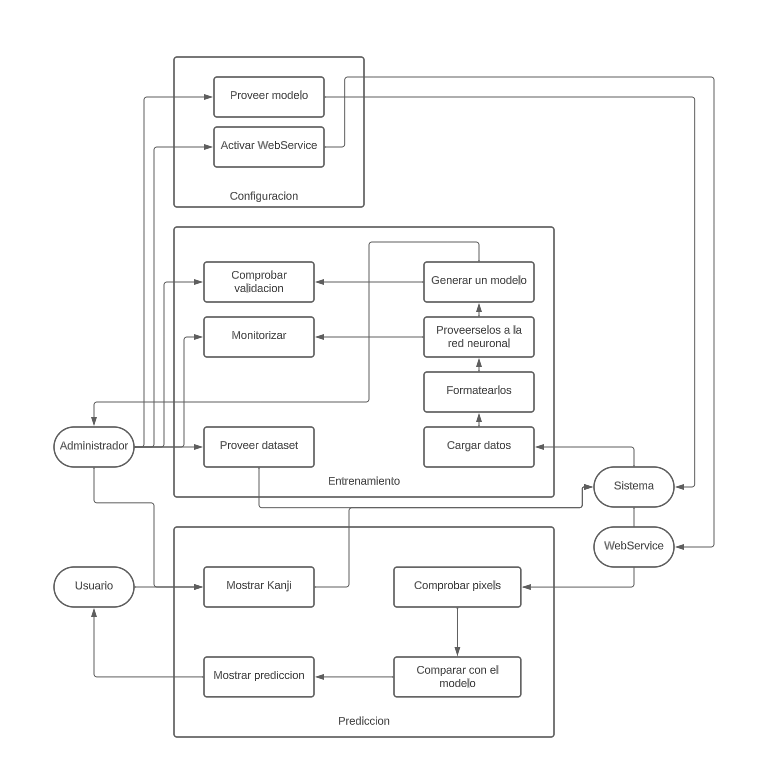
\includegraphics[width=1\textwidth]{pics/UseCases.png}
	\end{center}
   %\item Diagrama UML: Estado.
	\begin{center}
    	\centering
    	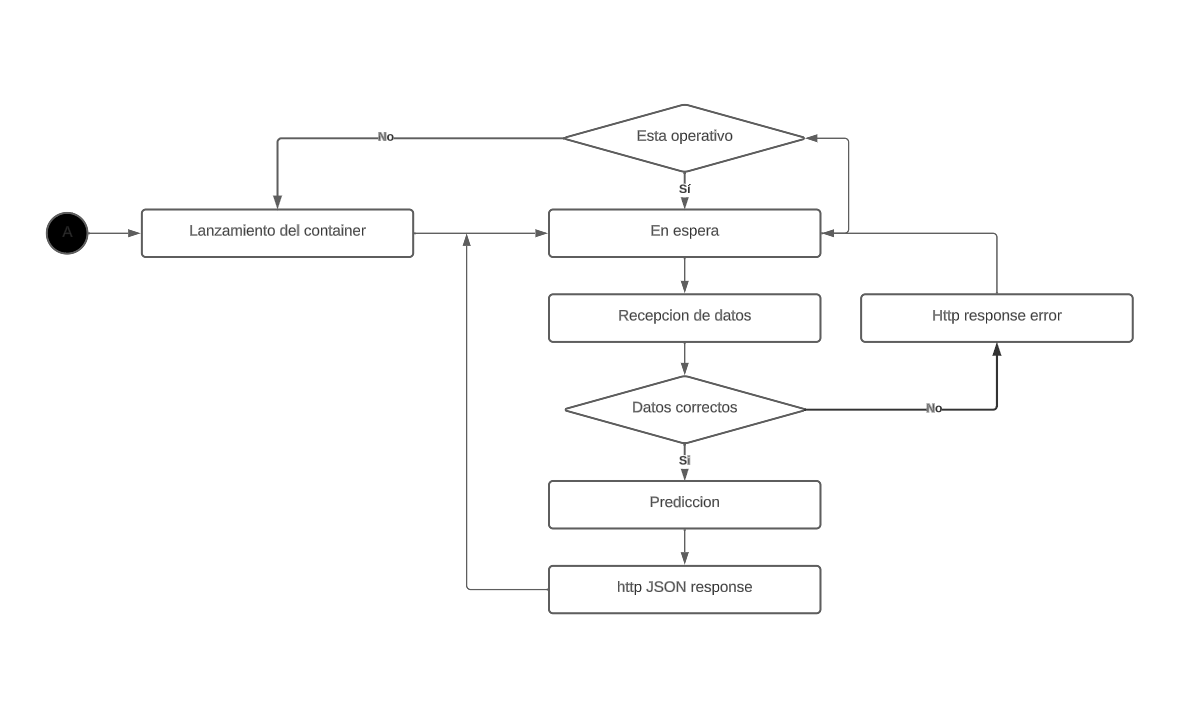
\includegraphics[width=1\textwidth]{pics/State.png}
	\end{center}
	%\item Diagrama UML: Despliegue.
	\begin{center}
    	\centering
    	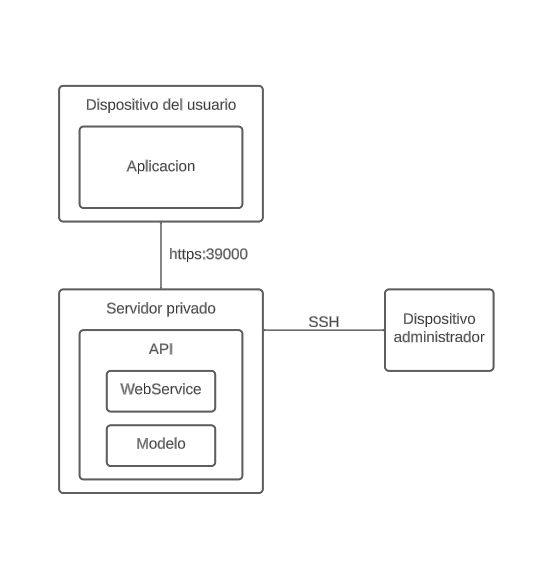
\includegraphics[width=0.7\textwidth]{pics/Deploy.png}
	\end{center}
	%\item Diagrama UML: Secuencia.
	\begin{center}
	\makebox[\textwidth]{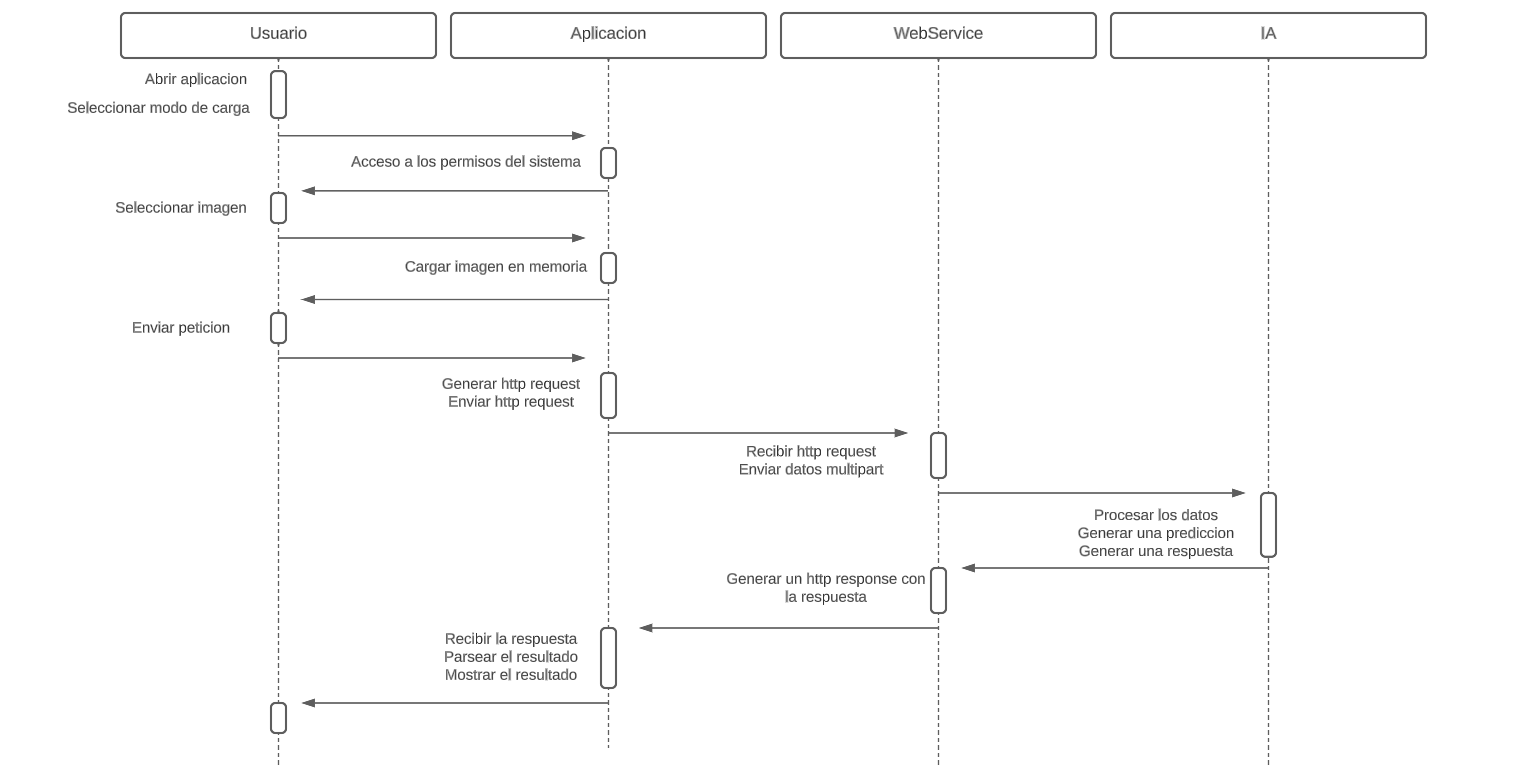
\includegraphics[width=\paperwidth]{pics/Sequence.png}}
	\end{center}
%\end{itemize}

\newpage
\subsection{Guía del desarrollador}
\label{sec:DevGuide}
\subsubsection{Configuración de Traefik}
\label{sec:Traefik}
Como se ha explicado previamente, para poder exponer nuestra aplicación a internet a través de nuestro servidor dockerizado, debemos configurar correctamente Traefik.

Sin entrar en demasiados tecnicismos, en este punto desarrollaremos cómo crear una configuración básica de Traefik con la que trabajar. Para más información, Traefik dispone de una amplia documentación online en la que solventar posibles dudas de funcionamiento y configuración.

En primer lugar, debemos crear una carpeta para el container de docker dentro de nuestro servidor, que almacenará el servicio Traefik y su configuración. En esta carpeta, crearemos un archivo \textit{docker-compose.yml} con la siguiente configuración:

\noindent\begin{minipage}{\textwidth}
\begin{lstlisting}
version: "3.7"
services:
	traefik:
    	image: traefik:2.4.8
    	container_name: traefik
    	networks:
        	- traefik-global-proxy
    	command:
        	- --entrypoints.http.address=:80
        	- --entrypoints.https.address=:443
        	- --providers.docker=true
        	- --providers.docker.network=traefik-global-proxy
        	- --providers.docker.exposedByDefault=false
        	- --api=true
        	- --certificateresolvers.letsencrypt.acme.httpchallenge=true
        	- --certificateresolvers.letsencrypt.acme.httpchallenge.entrypoint=http
        	- --certificateresolvers.letsencrypt.acme.email=#<email>
        	- --certificateresolvers.letsencrypt.acme.storage=/letsencrypt/acme.json
    	labels:
        	- traefik.enable=true
        	- traefik.http.routers.to-https.rule=HostRegexp(`{host:.+}`)
        	- traefik.http.routers.to-https.entrypoints=http
        	- traefik.http.routers.to-https.middlewares=to-https
        	- traefik.http.routers.traefik.rule=Host(`traefik.otterleek.com`)
        	- traefik.http.routers.traefik.entrypoints=https
        	- traefik.http.routers.traefik.middlewares=auth
        	- traefik.http.routers.traefik.service=api@internal
        	- traefik.http.routers.traefik.tls=true
        	- traefik.http.routers.traefik.tls.certresolver=letsencrypt
        	- traefik.https.middlewares.to-https.redirectscheme.scheme=https
        	- traefik.https.middlewares.auth.basicauth.users=leek:#<KEY>
    	ports:
        	-80:80
        	-443:443
    	volumes:
        	- ./data/letsencrypt: /letsencrypt
        	- var/run/docker.sock:/var/run/docker.sock:ro
networks:
	traefik-global-proxy:
    	name: "traefik-global-proxy"
\end{lstlisting}
\end{minipage}\\

Con esta configuración, y completando los puntos marcados con \#<...> con los parámetros correspondientes, se procede a levantar el container, y a través del docker compose y la configuración ya mencionados en esta guía con la que levantamos nuestro web service, la ruta especificada en este último ya entraría a través del dominio y los puertos especificados y, además, a través del protocolo https gracias a Let's Encrypt, una autoridad de certificación gratuita y para uso público.

De nuevo, como no es el propósito de este documento elaborar procesos de configuración detallados respecto a las herramientas externas utilizadas en el proyecto, cualquier información adicional puede obtenerse en la documentación oficial de Traefik.\\

\subsubsection{.README}
\begin{lstlisting}

## Documentation

[Docker](https://linktodocumentation)
[Traefik](https://linktodocumentation)
[FastAPI](https://linktodocumentation)
[Python](https://linktodocumentation)
[Debian](https://linktodocumentation)
[Flutter](https://linktodocumentation)
[Tensorflow](https://linktodocumentation)

## Requirements

### For running:
 - Docker or Python 3.8 installed on your machine

### For training:
 - Python 3.8
 - 32Gb RAM as it is, adaptable to run on 16Gb
 - 2Gb of storage available
 - Recommended Ryzen 5 5600 or higher
 * Note: Having a physical GPU available will decrease significantly the training times. It is recommended to have CUDA, although we include a package in requirements.txt that allows a translation from AMD Technology to CUDA (only for Windows OS)

## Run locally

To train the IA locally:

 - Clone the project
 - Install dependencies provided in `requirements.txt`
 - Download the dataset and the necessary fonts provided in the "necessary files" section
 - Unzip them in the root of the folder with the same name
 - Run the training_process.py script and wait for it to end


To run the IA locally without a container:

 - Clone the project
 - Install dependencies provided in `requirements.txt`
 - Run the main with uvicorn.


To deploy the IA locally end expose it to global network:

 - Follow the instructions provided in the section "Networking" of the documentation
 - Open the correct port
 - Clone the project
 - Create a container with the Dockerfile provided in the repository and the documentation
 - Run the container

 ## API Reference

#### Get a prediction

```https
  POST kanji.otterleek.ddns/
```

| Parameter | Type    	| Description            	|
| :-------- | :---------- | :------------------------- |
| `file`	| `multipart` | **Required**. Kanji image. |


\end{lstlisting}


\subsection{Agradecimientos}
\label{sec:Thanks}
Por último, quiero dedicar este pequeño fragmento a agradecer a toda la gente que ha hecho este proyecto posible. En primer lugar, a Jordi Amoros por sugerirme la idea, introducirme en el campo de la inteligencia artificial, y ayudarme con la revisión tanto del proyecto, como de esta documentación. En segundo lugar, a Vadim 'Ame' Perepelitsyn por guiarme en el proceso de networking y creación de containers, y finalmente a Javier Villegas por su ayuda en todo lo referente a estructuras de datos en python. Este proyecto hubiese sido prácticamente imposible sin vuestro apoyo.

Un agradecimiento también a todo mi entorno, profesorado, familia y amigos, que me han ayudado y apoyado durante el curso y el desarrollo del proyecto.

Gracias a todos.

\newpage

\section{Bibliografía}
\label{sec:bib}










\begin{comment}
\documentclass{article}


%Page design
\usepackage[letterpaper, top=0.7in, bottom=0.7in, left=1.0in, right=1.0in, heightrounded]{geometry}

%Budget
\usepackage{booktabs}
\usepackage{longtable}
\usepackage{tabularx}
\usepackage{eurosym}

%Maths
\usepackage{graphicx}
\usepackage{amsmath, amssymb, amsthm}

%Formatting
\usepackage{xcolor}
\usepackage{tabto}
\usepackage{indentfirst}
\usepackage[square,numbers]{natbib}
\usepackage[T1]{fontenc}   
\usepackage[labelformat=empty]{caption}

%Footers
\usepackage{footmisc}
\usepackage{fixfoot}

%Bibliography
\bibliographystyle{abbrvnat}

%Code displaying
\usepackage{verbatim}
\usepackage{listings}
\usepackage{xcolor}
\usepackage[square,numbers]{natbib}

\definecolor{codegreen}{rgb}{0,0.6,0}
\definecolor{codegray}{rgb}{0.5,0.5,0.5}
\definecolor{codepurple}{rgb}{0.58,0,0.82}
\definecolor{backcolour}{rgb}{0.95,0.95,0.92}

\lstdefinestyle{mystyle}{
    backgroundcolor=\color{backcolour},   
    commentstyle=\color{codegreen},
    keywordstyle=\color{magenta},
    numberstyle=\tiny\color{codegray},
    stringstyle=\color{codepurple},
    basicstyle=\ttfamily\footnotesize,
    breakatwhitespace=false,         
    breaklines=true,                 
    captionpos=b,                    
    keepspaces=true,                 
    numbers=left,                    
    numbersep=5pt,                  
    showspaces=false,                
    showstringspaces=false,
    showtabs=false,                  
    tabsize=2
}
\lstset{style=mystyle}

%Index
\usepackage[hidelinks]{hyperref}
\usepackage{imakeidx}
\makeindex[columns=3, title=Indice, intoc]

%Lengths and spacing
\setlength{\skip\footins}{20pt}
\setlength{\parindent}{1cm}
\setlength{\parskip}{1pt}
\newcommand\mytab{\tab \hspace{-5.5cm}}
\renewcommand{\baselinestretch}{1.15}

%Fixed footnotes
\DeclareFixedFootnote{\tec}{Definiciones en \hyperref[sec:terms]{Anexo 1: Términos tecnicos}}
\DeclareFixedFootnote{\iae}{Más detalles en los documentos del Anexo 2: Información adicional externa.}
\DeclareFixedFootnote{\mnn}{Explicaciones pertinentes en el Anexo 4: IA: Modelo y Neural Network}
\DeclareFixedFootnote{\gdd}{Más detalles en el Anexo 5: Guía del desarrollador}

%Fix hyphenation
\tolerance=1
\emergencystretch=\maxdimen
\hyphenpenalty=10000
\hbadness=10000

%%%%%%%%%%%%%%%%%%%%%%%%%%%%%%%%%%%%%%%%%%%%%%%%%%%%%%%%%%%%%%%%%%%%%%%%%%%%

\graphicspath{./pics/}
\title{Proyecto Final CFGS Desarrollo de Aplicaciones Muliplataforma}
\author{Carlos Manso}
\date{2023 - 2024}
%%%%%%%%%%%%%%%%%%%%%%%%%%%%%%%%%%%%%%%%%%%%%%%%%%%%%%%%%%%
%%%%%%%%%%%%%%%%%%%% PROYECTO FINAL %%%%%%%%%%%%%%%%%%%%%%%
%%%%%%%%%%%%%%%%%%%%%%%%%%%%%%%%%%%%%%%%%%%%%%%%%%%%%%%%%%%

\begin{document}
\clearpage\maketitle
\thispagestyle{empty}

\setcounter{tocdepth}{2}
\clearpage\tableofcontents
\thispagestyle{empty}
\pagenumbering{arabic}
\newpage

%%%%%%%%%%%%%%%%%%%% INTRODUCCION %%%%%%%%%%%%%%%%%%%%%%%

\section{Introducción}
\label{sec:Intro}


%TODO: Seleccionar acentos españoles para poder tildar las palabras y poner Ñs

\subsection{Origen}
La elección de este proyecto surge después de una intensa búsqueda de ideas entre las que se encuentran proyectos como una aplicación de estudios, un videojuego, un motor gráfico, una aplicación de memorización... Proyectos que me atraían para desarrollar, pero que no veía con tanto uso en el futuro como la opción finalmente elegida. 

El proyecto consiste, en su forma más conceptual, de una inteligencia artificial capaz de predecir un \hyperref[sec:terms]{\textit{kanji}\tec} a través de su imagen, ya sea caligrafiado o impreso, y devolver dicho kanji en texto copiable para poder usarlo, buscarlo, o reconocerlo con mayor facilidad.

El resultado que les muestro en la memoria a continuación no ha sufrido grandes modificaciones en el desarrollo y las metas que se pretendían seguir con el mismo, manteniéndose bastante fiel a la idea original, aunque sí que se han tenido que adaptar ciertos aspectos que se comentarán mas adelante en esta memoria.

\subsection{Motivacion}
Personalmente disfruto del ámbito del \hyperref[sec:terms]{\textit{data science}\tec}, los idiomas y desarrollar mis propias herramientas en la medida de lo posible, por lo que desarrollar una utilidad como la descrita era un paso lógico a tomar en algún momento. Como estudiante de japonés, conozco de primera mano el valor que una herramienta así puede suponer para los estudiantes de este idioma.

Además, es un proyecto muy extendible, tanto a través de nuevas funcionalidades no contempladas en el desarrollo inicial, como extendiendo su funcionamiento a otros idiomas de alfabeto no romano.

\subsection{Comentario del autor}
Este documento esta pensado para que cualquier persona pueda entender el desarrollo en términos generales, por lo que los tecnicismos o anglicismos que se utilizan estarán definidos en uno de los anexos. No obstante, cabe mencionar que se da por sentado un conocimiento mínimo de informática en el lector para poder entender al completo todas las explicaciones que se desarrollan a continuación, ya que abarca tanto el objetivo del proyecto y sus motivaciones y planificaciones, como su puesta en marcha, funcionamiento y guías para desarrolladores y usuarios. Asimismo, el objetivo de este documento tampoco abarca las explicaciones sobre diversos conceptos a bajo nivel, funciones matemáticas, y otros conceptos avanzados necesarios para el desarrollo del proyecto que se presenta, que ya se encuentran desarrollados en las herramientas utilizadas. Para mas información al respecto, se facilitan algunas fuentes para su consulta en los anexos correspondientes.


%%%%%%%%%%%%%%%%%%%% CONTEXTUALIZACION %%%%%%%%%%%%%%%%%%%%%%%
\newpage

\section{Contextualización}
\label{sec:Context}

\subsection{Necesidad}
En los ambitos personal y social, una herramienta capaz de transformar la imagen de un kanji complejo en un caracter \hyperref[sec:terms]{\textit{Unicode}\tec} legible por cualquier persona y copiable en un dispositivo, es de gran utilidad para el estudio del idioma. Algunos estilos de escritura o ciertos documentos antiguos no guardan casi ningún parecido con la forma de escribir los kanji a día de hoy, especialmente a la hora de comparar caligrafía humana con caracteres digitales.

Uno de los problemas mas comunes para los estudiantes de este idioma es reconocer kanjis, ya que se trata de un alfabeto de mas de 3000 caracteres distintos, cada uno con varias lecturas, y que pueden combinarse para formar significados y lecturas nuevas. 

Aunque las combinaciones son mucho mas complejas de cotejar y requieren de un estudio y una comprensión extensa de los caracteres individuales, una aplicación que nos facilite la tarea de reconocerlos de forma aislada supone una gran herramienta, ya que en numerosas ocasiones, poder reconocerlos por separado es suficiente para contextualizar la combinación y conocer el significado de ésta.

Es en este punto donde entra en juego mi proyecto, ofreciendo una forma sencilla de reconocer caracteres kanji que el usuario pueda ver en cualquier tipo de multimedia o en formato físico. A traves de una captura de pantalla o una fotografía del caracter, podra obtenerlo en un formato digital mucho mas comprensivo y versátil para su identificación o para buscar información al respecto.

\subsection{Objetivo}
El proyecto esta, lógicamente, limitado en cierta forma tanto por el tiempo disponible para su desarrollo como por la capacidad de computación a la que tengo acceso en la actualidad para el entrenamiento del \hyperref[sec:terms]{\textit{modelo}\tec}. 

No obstante, aunque existen Inteligencias Artificiales (de ahora en adelante \hyperref[sec:terms]{\textit{IAs}\tec}) a día de hoy muy perfeccionadas como puede ser la de Google, parte del objetivo del proyecto es el de crear la propia herramienta desde cero, introduciéndome en un nuevo ámbito de la programación. 

La mayoría de recursos con una funcionalidad similar a la que yo presento, no disponen de una aplicación particular para ello, no son fácilmente escalables, o requieren que el propio usuario intente plasmar el caracter a mano para su reconocimiento. Esto último supone un problema, ya que por una parte, ciertos kanjis son demasiado complejos para ser copiados a mano por el usuario; y por otra, estos métodos de reconocimiento tienen en cuenta el orden de los trazos, esto quiere decir, que por como son las reglas caligráficas del kanji, intentar plasmar el mismo caracter variando el orden de los trazos puede dar diferentes resultados.

El objetivo general es, por tanto, generar una IA y una aplicación a través de las cuales se pueda introducir la imagen de un kanji aislado, y nos devuelva el kanji de la imagen en un caracter Unicode copiable.

%%%%%%%%%%%%%%%%%%%% OBJETIVOS %%%%%%%%%%%%%%%%%%%%%%%
\newpage

\section{Objetivos específicos}
\label{sec:Objectives}

Los objetivos específicos del proyecto se desgranan en los siguientes puntos:

\begin{itemize}
    \item Desarrollar un modelo de IA capaz de reconocer caracteres para entender el funcionamiento elemental de un algoritmo de reconocimiento de caracteres.
    \item Desarrollar un modelo capaz de entrenar y reconocer caracteres japoneses, tanto escritos a mano como digitales con un porcentaje de acierto suficiente como para ser de utilidad.
    \item Crear una \textit{Application Programming Interface} \hyperref[sec:terms]{(\textit{API}\tec)} capaz de recibir imágenes de kanjis y devolver sus predicciones.
    \item Alojar la API en un servidor privado y exponerla a internet para poder consumir el servicio desde diferentes dispositivos en cualquier lugar donde dispongamos de acceso a internet.
    \item Desarrollar una interfaz gráfica de usuario con la que podamos tomar o cargar imágenes y enviarlas a un \hyperref[sec:terms]{\textit{web service}\tec} que crearemos para que nos devuelva una predicción a dicha interfaz.
\end{itemize}

Las tareas a desarrollar se describen en mayor detalle en la siguiente sección, así como los detalles sobre los procesos utilizados, resultados, código fuente, etc. También se podrá encontrar documentación adicional a todos estos procesos en los anexos correspondientes.

%%%%%%%%%%%%%%%%%%%%%%%%%%%%%%%%%%%%%%%%%%%%%%%%%%%%%%%%%%%
%%%%%%%%%%%%%%%%%%%% PROYECTO FINAL %%%%%%%%%%%%%%%%%%%%%%%
%%%%%%%%%%%%%%%%%%%%%%%%%%%%%%%%%%%%%%%%%%%%%%%%%%%%%%%%%%%


\section{Tareas}
\label{sec:Tasks}

Respecto a las tareas a realizar a nivel de proyecto para poder llevar a cabo los objetivos mencionados en el punto anterior, se plantean cuatro puntos bien diferenciados, que se desgranan a su vez en diferentes subtareas. La lista de tareas viene especificada a continuación, y desarrollada en la \hyperref[sec:Development]{sección 5}, donde se explica cada una de forma detallada.

\begin{itemize}
    \item Modelo de prueba
    \item Entrenamiento del modelo
    \begin{itemize}
        \item Elección de librerías
        \item Búsqueda del \hyperref[sec:terms]{\textit{dataset}\tec}
        \item Diseño de la \hyperref[sec:terms]{\textit{red neuronal}\tec}
        \item Diseño del entrenamiento
        \item Validación
    \end{itemize}
   \item Implementación
    \begin{itemize}
        \item Configuración de los métodos
        \item Presentación del resultado
    \end{itemize}
   \item Alojamiento
    \begin{itemize}
        \item Montaje e instalación del servidor
        \item Networking
        \item Dockerización
    \end{itemize}
    \item Creación de la interfaz
    \begin{itemize}
        \item Frontend
        \item Backend
    \end{itemize}
\end{itemize}


\section{Desarrollo}
\label{sec:Development}

\subsection{Modelo de prueba}
\begin{comment}
La idea es realizar un modelo basico de inteligencia artificial capaz de clasificar correctamente imagenes de dígitos para familiarizarme con el lenguaje y con los tipos y formatos de datos con los que tendre que trabajar durate el desarrollo. 
    
Para realizar este punto, se busca una guia paso a paso sobre como realizar una IA muy basica llamada \textit{Clasificador KNN}\tec\space de reconocimiento de digitos, sin embargo, como no es el punto original de este proyecto, no vamos a desarrollar en detalle el proceso de creacion.
Esencialmente, el algoritmo se encarga de realizar predicciones basadas en el análisis de los datos que se le pasan y los datos de los que dispone en su dataset local, mirando las instancias mas cercanas, y calculando una media, prediciendo aquel o aquellos resultados mas cercanos al dato analizado. Este proceso lo realiza cada vez que se le solicita una prediccion.
    
En las pruebas realizadas se registro un ratio de acierto del 100\%, con 12 imagenes tanto pertenecientes al dataset como dibujadas por el usuario, con una certeza de acierto de en torno al 80\% en sus niveles mas bajos. Se incluye el codigo de este algoritmo en el Anexo 3, pero como ya hemos comentado, no entraremos en mas detalle al respecto, puesto que no tiene estricta relacion con el proposito del proyecto.
end{comment}
La idea es realizar un modelo básico de IA capaz de clasificar correctamente imágenes de números para familiarizarme con el lenguaje y con los tipos y formatos de datos con los que se tendrá que trabajar durate el desarrollo. 

Cabe mencionar que esta parte del proyecnto tiene una fase previa de investigar y documentarnos acerca de qué lenguaje utilizaremos para esto. En el momento del desarrollo, la herramienta mas utilizada para creacion de IAs es Python 3, por lo que de este punto inclusive en adelante, será el lenguaje que usaremos para nuestro desarrollo, salvo que se indicase lo contrario de forma específica.
    
Para realizar este punto, se busca una guia paso a paso sobre como desarrollar una IA muy basica llamada \hyperref[sec:terms]{\textit{Clasificador KNN}\tec} de reconocimiento de numeros, sin embargo, como no es el objetivo original de este proyecto, no vamos a desarrollar en detalle el proceso de creacion. 
    %TODO: Cambia la referencia del anexo 3
En las pruebas realizadas se registro un ratio de acierto del 100\%, con 12 imagenes tanto pertenecientes al dataset como dibujadas por el usuario. En el parametro de certeza (encargado de medir el nivel de confianza en la predición proporcionada) se obtienen resultados en torno al 80\%. Se incluye el codigo de este algoritmo en el \hyperref[sec:terms]{\textit{anexo 3}}, pero como ya hemos comentado, no entraremos en mas detalle al respecto, puesto que no tiene estricta relacion con el proposito del proyecto.

\begin{figure}[!ht]
    \centering
    \label{fig:mnist}
    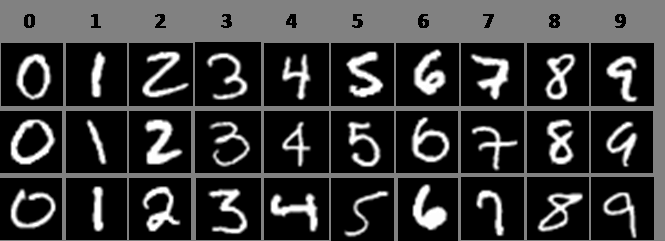
\includegraphics[scale=0.5]{pics/mnist_numbers.png}
    \caption{Ejemplo de input para entrenamientos y validaciones del KNN}
\end{figure}



\subsection{Entrenamiento del modelo}
Una vez finalizada la prueba de concepto, se comienza con el desarrollo del modelo, esto es, su proceso de creacion, entrenamiento, validacion, uso, etc. Para ello debemos subdividir esta seccion en varias partes que, no obstante, estan interrelacionadas, y por tanto pueden verse afectadas entre sí. A continuación se explican cada una de estas subtareas:

\subsubsection{Eleccion de librerias}
Existen ciertas librerias basicas de las que debemos partir. Para ello debemos realizar un estudio sobre las tecnologias y procesos que necesitaremos, qué funcionalidades vamos a desarrollar y de qué herramientas necesitaremos disponer. No obstante, a lo largo del desarrollo podremos ir necesitando librerias adicionales con las que no hayamos contado en primer lugar que habra que tener en cuenta a la hora de documentar el proyecto.

En nuestro caso, se contempla inicialmente la posibilidad de utilizar PyTorch, una libreria de IA bastante conocida y con amplia trayectoria, pero tras navegar a traves de la documentacion e informarme a traves de diversas fuentes, se decide finalmente utilizar la libreria de Tensorflow, debido a, entre otros motivos, una mayor facilidad de uso de su API, una documentacion mas extensa y explicativa, y mayor uso entre los desarrolladores actuales de IAs, lo que se traduce en mayor contenido e informacion respecto a los diversos problemas y opciones con las que nos enfrentamos durante el desarrollo.

Adicionalmente a la libreria de Tensorflow, conocemos ciertas librerias que necesitaremos usar con seguridad a lo largo del desarrollo como PIL(Pillow) para manejo de imagenes, matplotlib para generacion de graficos informativos, Keras como anexo a Tensorflow para el entrenamiento, numpy para creacion de matrices y otras colecciones con el poder computacional que ofrece C, y muy importante, torch-directml para integrar entrenamientos de IA con graficas de AMD a traves de Direct-X12.

\subsubsection{Busqueda del dataset}
Parte esencial de la creacion de una IA, es utilizar un dataset adecuado, por lo que, a falta de capacidad y tiempo para generar uno propio, debemos buscar un dataset ya existente con los contenidos que necesitemos y, de ser necesario, adaptarlo a nuestras necesidades.

\begin{comment}
La eleccion del dataset se ve condicionada por la escasez de ellos. Esencialmente, podemos encontrar dos datasets distintos en todo internet, el primero siendo Kuzushiji-Kanji, que es el que finalmente se utilizara en este proyecto tras sopesar ventajas e inconvenientes, y ELTCDB. Aunque el primero es un dataset mucho mas desfasado, incompleto y desbalanceado, viene muy convenientemente clasificado y listo para su uso, mientras que el segundo viene subdividido en diversos sets de caracteres, y con sus imagenes convertidas en formato binario anexadas unas detras de otras, que habria que tratar correctamente bajo estrictas instrucciones proporcionadas por el AIST (National Institute of Advanced Industrial Science and Technology). 

Debido a esto, aunque la eficacia de la IA se vera mermada por la integridad del dataset, la implementacion del modelo puede hacerse casi de forma directa a traves de la API de Keras.
Para compensar este desbalance del dataset, se crean dos programas .py. En el primero, generamos, en base a diferentes fuentes en japones, una imagen acorde al formato de las imagenes de nuestro dataset de cada uno de los kanji pertenecientes al JLPT y la anadimos al dataset. En el segundo, recorreremos de nuevo nuestro dataset y eliminaremos de este todas las carpetas e imagenes de kanjis que se repitan menos de 5 veces, ya que consideramos que es un minimo a partir del cual el hecho de que ese kanji exista en el modelo, produce mas falsos resultados que resultados correctos sin importar las correcciones que intentemos aplicarle.
end{comment}
La elección del dataset se ve condicionada por la escasez de éstos. Esencialmente, podemos encontrar dos datasets distintos en internet. 

El primero es ELTCDB, que aunque a primera vista tiene una mejor calidad de datos, éstos vienen en un formato más incómodo para trabajar con el. Esencialmente, debes pedir permiso al AIST (National Institute of Advanced Industrial Science and Technology) para obtener acceso, y una vez concedido, todos los datos se encuentran en binario, subdivididos de forma irregular y bajo un estándar propio del AIST, quien te proporciona las instrucciones para decodificarlos correctamente. 

Es por la complejidad en el proceso de obtener los datos en el formato que queremos, que se opta por la segunda opcion: Kuzishiji-Kanji, que sí que viene en un formato conveniente para nuestro caso de uso. Como inconveniente de este dataset, cabe destacar que sus datos estan ligeramente mas desfasados, es algo mas incompleto y está peor balanceado.

Sin embargo, aunque la eficacia de la IA se vera mermada por la integridad del dataset, elegimos este dataset, ya que la implementacion del modelo puede hacerse casi de forma directa a traves de la API de Keras.

Para compensar este desbalance del dataset, se crean tres scripts:
\begin{itemize}
    \item El primero genera, en base a diferentes fuentes en japonés, una imagen acorde al formato de las imagenes contenidas en nuestro dataset por cada kanji disponible para aumentar el numero de muestras.
    \item El segundo se encarga de recorrer de nuevo el dataset, eliminando todas las carpetas e imagenes que contengan menos de diez muestras, el minimo que consideramos para obtener un resultado consistente. Esto se hace teniendo en cuenta que el anterior script generará aproximadamente, 7 muestras por kanji.
    \item El tercero se encarga de normalizar el numero de muestras. Lo ideal es que se entrene bajo un rango sin una gran discrepancia entre mayor y menor numero de muestras. Para esto, en nuestro script se generan por data augmentation nuevas muestras en aquellos kanji por debajo de un umbral minimo, y se eliminan muestras aleatorias en aquellos por encima de un umbral maximo. En nuestro caso, los umbrales se situan en 500 muestras máximo, y 80 mínimo.
\end{itemize}
Cabe destacar que los kanji en los que ocurre esto son, generalmente, muy poco comunes de ver, o que han caido en desuso.

\subsubsection{Diseño de la red neuronal}

Es importante realizar un estudio en profundidad de los disenos de redes neuronales recomendables para la funcionalidad que estamos buscando, y, posteriormente, analizar los resultados de la \hyperref[sec:terms]{\textit{validacion}\tec} y realizar pruebas de los modelos generados utilizando esta red para poder ajustar sus parametros de configuracion acorde con el dataset que le vamos a proporcionar.\\

\noindent Antes de comenzar con explicaciones más técnicas, conviene conocer la siguiente terminología:
\begin{itemize}
    \item Capa: Una capa es el bloque mas general dentro de un modelo de IA. Son contenedores que se encargan de recibir un dato de entrada, transformarlo a partir de determinadas operaciones matematicas, y generar un dato de salida con el que informar a la siguiente (o generar un resultado final en el modelo). Las capas se dividen en \textit{input} y \textit{output layers}, siendo respectivamente la primera y la ultima capa del modelo, y \textit{hidden layers} siendo estas todas las que se encuentren entre las dos anteriores.
    \begin{figure}[!ht]
        \centering
        \label{fig:cnn}
        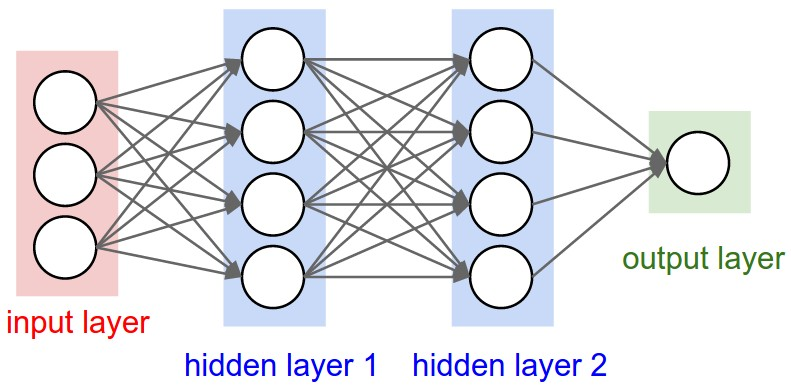
\includegraphics[scale=0.25]{pics/cnn.jpg}
        \caption{Estructura de capas en una red neuronal.}
    \end{figure}
    \item Convolucion: Se trata de una operación matematica que describe como fusionar dos partes de informacion, primero un dato de entrada (en nuestro caso concreto, el valor de cada píxel), y segundo el valor conjunto de todos los vecinos definidos por el kernel, para generar un mapa de caracteristicas del dato inicial.
    \item Kernel: consiste en una pequena matriz que itera sobre los datos de entrada, realizando determinadas operaciones entre el elemento seleccionado y los elementos de su alrededor y calculando un nuevo resultado para el elemento original.
    \begin{figure}[!ht]
        \centering
        \label{fig:conv}
        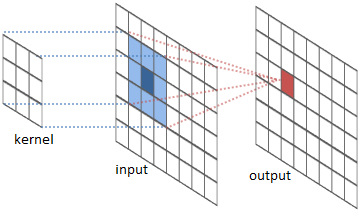
\includegraphics[scale=0.5]{pics/convolution.png}
        \caption{Proceso de convolución de una imagen}
    \end{figure}
    \item Neurona: Al nivel mas conceptual, una neurona es una funcion que opera sobre los datos de entrada ($x_n$), aplicándole unos pesos ($w_n$), y dando como resusltado una salida ($y$) que puede ser procesada por una función de activación. Generalmente, cada una de estas unidades, se encuentra conectada en ambos sentidos a varias neuronas. Estas unidades pueden seguir diferentes patrones de conexion entre ellas o ser usadas en conjunto con múltiples funciones de activación.
    \item Peso: Son valores numéricos que se asocian a las conexiones entre las neuronas de diferentes capas. Estos se inicializan de forma aleatoria con la primera iteración del entrenamiento, y a partir de una serie de ecuaciones, son ajustados para las siguientes iteraciones acorde a los resultados obtenidos.
        \begin{figure}[!ht]
        \centering
        \label{fig:perceptron}
        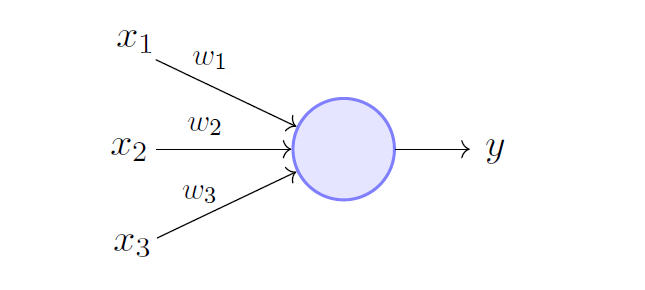
\includegraphics[scale=0.4]{pics/perceptron.png}
        \caption{Representación del funcionamiento de una neurona}
    \end{figure}
    \item Activación: Las funciones de activacion son operaciones matematicas que se encargan de  transmitir la información generada por la neurona a las neuronas de la siguiente capa. La funcion de activacion puede ser de muchos tipos según el resultado que se pretenda obtener. Algunos de estos tipos son Sigmoid (transformar los valores introducidos a una escala 0-1), Softmax (transformar el sumatorio de todas las salidas a 1) y que se utilizara en otros puntos relevantes del proyecto, o ReLU, como utilizamos en este caso (transformar los valores de entrada anulando los negativos y dejando los positivos sin modificar). En terminos generales, se buscan funciones cuyas derivadas sean simples para minimizar al maximo el coste computacional del entrenamiento.

\end{itemize}

Vistos los términos mas comunes que utilizaremos en nuestra explicación, los detalles específicos para nuestro proyecto se describen a continuación.

Se ha optado por un diseño de red convolucional (explicado mas adelante) que sigue un patrón bastante extendido y recomendado para IAs cuyo objetivo es \textit{Optical Character Recognition} (\hyperref[sec:terms]{\textit{OCR}\tec}), como es nuestro caso. 

En los párrafos a continuación, se procede a profundizar de forma más tecnica este diseño, no obstante cabe destacar que no se ofrecen una gran cantidad de detalles con respecto a las propiedades de las herramientas que utilizamos, ya que son de una gran complejidad y se salen del objetivo de este documento.\\

Nuestra red neuronal esta compuesta por dos bloques principales. Un primer bloque compuesto por capas de Convolucion y Pooling que se encargarán de extraer información de las imágenes, y un segundo bloque compuesto por capas Densas.

Previo a las capas definidas a continuación, se aplican dos transformaciones extra, una de redimension, y una de reescalado, que transformarán los datos introducidos al modelo al tamaño y formato de datos requeridos por la capa inicial. 

Las capas convolucionales se encargan de extraer la información relevante de la imagen a través de la iteración de un kernel por cada pixel de la imagen. Esto dará como resultado una imagen del mismo tamaño que la original donde cada pixel tendrá la información relevante sobre aquellos a su alrededor.

Las capas de MaxPooling2D, al igual que las Convolucionales, iteran un kernel por cada pixel de la imagen, pero al contrario que éstas ultimas, su objetivo es reducir el tamaño total de la imagen descartando los resultados menos relevantes, ayudando al modelo a  centrarse en las características de mayor importancia y reduciendo el tiempo de procesamiento.

A continuacion de este grupo de capas, interviene una capa de Dropout, que fuerza al modelo a ignorar cierta cantidad de neuronas que se eligen de forma aleatoria en cada iteracion del entrenamiento, de forma que se incentiva a la red a buscar caminos alternativos para la resolucion del problema planteado. Esto previene que el algoritmo genere una dependencia a ciertas neuronas, reduciendo el \hyperref[sec:terms]{\textit{overfitting}\tec} y mejorando la capacidad de respuesta a nuevos datos.

\begin{figure}[!ht]
    \centering
    \label{fig:model}
    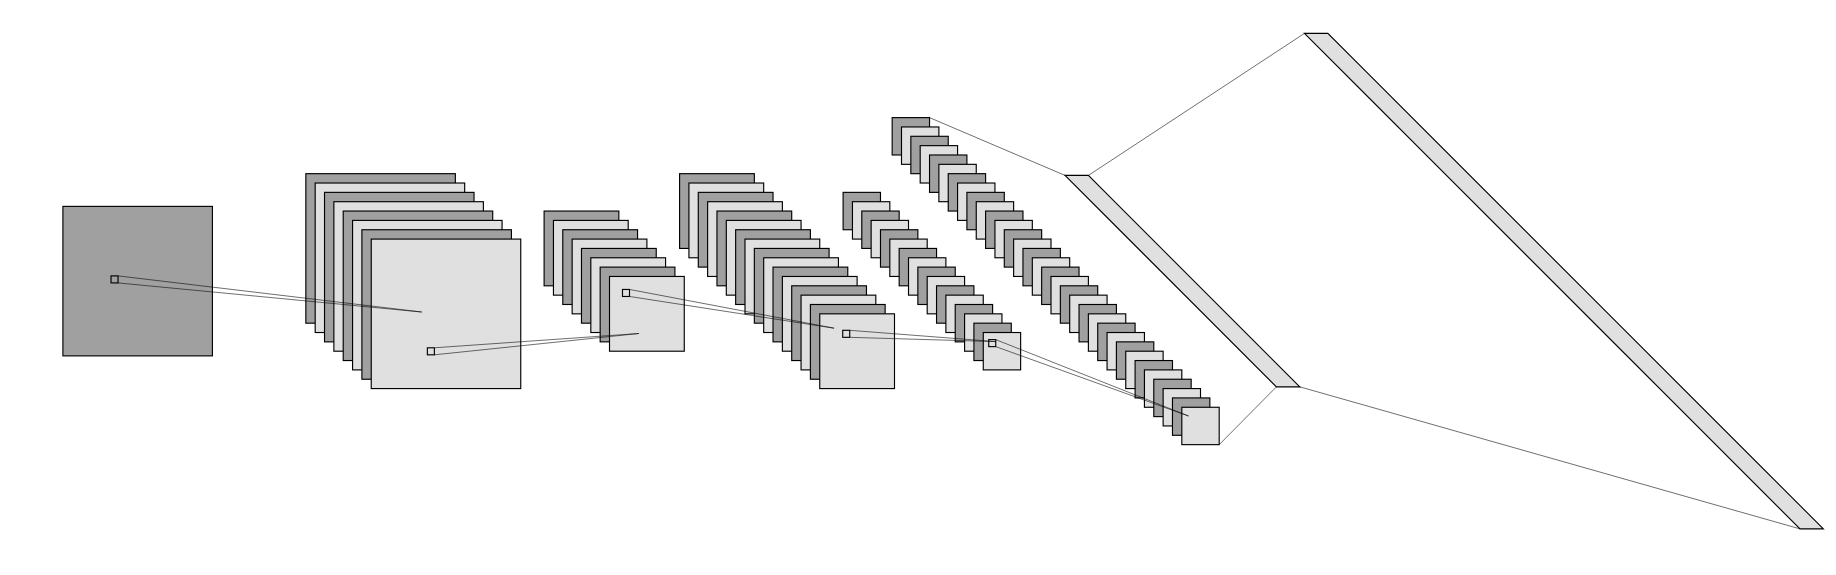
\includegraphics[scale=0.3]{pics/LeNetStyle.png}
    \caption{Representacion LeNet de nuestro modelo}
\end{figure}

A traves de una capa Flatten, simplemente transformamos los datos que hemos obtenido con las funciones anteriores en una secuencia lineal de forma que sea mas simple para el algoritmo conectar los datos y entender el conjunto global de la imagen original en las siguientes capas del modelo.

Llegando al final del modelo, disponemos dos capas densas, intercaladas por otra capa Dropout. Las capas densas son aquellas donde el modelo pasa de analizar los datos a clasificarlos, para en la última capa generar un resultado final. En estas capas, cada neurona de la capa actual, esta conectada a cada una de las neuronas de la capa anterior, y estas conexiones llevan asociadas un peso ajustado durante el entrenamiento. Son capas particularmente utiles en el reconocimiento de patrones. A las neuronas de estas capas tambien se les aplica una funcion de activacion ReLU, que permite a la red aprender relaciones complejas entre los datos. La salida de datos tras pasar por este modelo viene directamente de la ultima capa densa, cuyo numero de neuronas es igual al numero de kanji disponibles en nuestro dataset. El valor de salida de cada una de las neuronas de la última capa, representará la probabilidad de que el kanji asociado a dicha neurona sea el mismo que el de el dato de entrada.

Tambien es importante remarcar que lo anterior es una explicacion general del diseño y funcionamiento del modelo, realizado con una libreria de alto nivel. El funcionamiento de esta NN y las funciones que lo componen es mucho mas compleja y tecnica de lo que se pretende explicar en esta documentacion. Toda informacion al respecto puede obtenerse en la documentacion oficial de Tensorflow.\\

\noindent\begin{minipage}{\textwidth}
\begin{lstlisting}[language=python]
model = Sequential([
    tf.keras.Sequential([
        layers.Resizing(64, 64),
        layers.Rescaling(1./255)
    ]),
    layers.Conv2D(16, 3, padding='same', activation='relu'),
    layers.MaxPooling2D(),
    layers.Conv2D(32, 3, padding='same', activation='relu'),
    layers.MaxPooling2D(),
    layers.Conv2D(64, 3, padding='same', activation='relu'),
    layers.MaxPooling2D(),
    layers.Dropout(0.2),
    layers.Flatten(),
    layers.Dense(128, activation='relu'),
    layers.Dropout(0.2),
    layers.Dense(len(labels), name='outputs')
])
\end{lstlisting}
\end{minipage}\\\\\\


\subsubsection{Declaracion del modelo}

\noindent\textbf{Terminologia}
\begin{itemize}
    \item Batch: Se trata de un parametro que se encarga de determinar el numero de datos que se cargaran en memoria por cada iteracion de la epoca actual del entrenamiento. Cuanto menor sea este numero, mas ruido se generara en el entrenamiento, pero mucho menor seran los recursos utilizados.
    \item Época: Se trata de un ciclo completo a través de todo el conjunto de datos de entrenamiento. El numero de épocas indica la cantidad de iteraciones que el algoritmo de aprendizaje completará a lo largo de un proceso de entrenamiento.
    \item Funcion de perdida: Es la funcion que se encarga de medir como de precisas son las predicciones que realice nuestro modelo con respecto a los resultados veridicos. El objetivo es conseguir que su resultado sea lo menor posible, es decir, que el ratio de error sea lo mas pequeño posible. Aunque existen multiples funciones de perdida como Hinge Loss (clasificacion binaria) o Mean Absolute Error (error promedio en tareas simples de regresion), en este caso se ha utilizado Categorical Cross-entropy, disenada para tareas de clasificacion multiclase, en la que se analizan las diferencias entre las probabilidades de la prediccion y el valor real.
    \item Optimizador: Se trata de un algoritmo que se encarga de ajustar ciertos parametros internos del modelo durante su entrenamiento, buscando minimizar el ratio de error, optimizando los pesos en base a los resultados de la funcion de perdida aplicada al modelo. Existen numerosos algoritmos de optimizacion, y su eleccion dependera de diversos factores como la velocidad de convergencia que queramos obtener, como de eficiente en terminos de memoria queramos que sea, o los tipos de datos de entrada, entre otros. Algunos de los mas utilizados son SGD(-Stochastic Gradient Descent-, que opimiza en base al gradiente general del modelo), RMSProp(-Root Mean Scope Propagation-, que optimiza en base al gradiente medio de los resultados mas recientes), Momentum(que toma como base SGD, pero teniendo en cuenta tambien la media global en lugar de los resultados individuales), Adam(-Adapting Moment Estimation- que ajusta individualmente los parametros combinando los algoritmos de RMSProp y Momentum)...
    \item Gradiente: Es un vector calculado en base a las derivadas parciales de nuestra funcion de perdida y nuestro ratio de aprendizaje. Simplificando, es una guia que utiliza nuestro algoritmo para modificar sus pesos de forma dinamica y generar mejores resultados, es decir, si nuestro objetivo es llegar al punto 0 en una curva descendente de errores, el gradiente seria la verticalidad de la pendiente de la curva.

\begin{figure}[!ht]
    \centering
    \label{fig:gradex}
    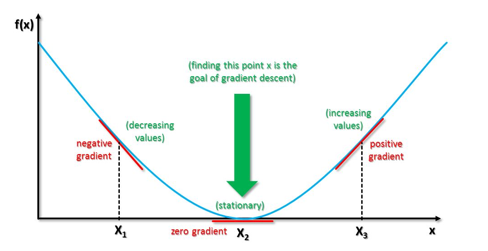
\includegraphics[width=0.7\textwidth]{pics/gradexp.png}
\end{figure}
    
    \item Momentum: Aunque se ha mencionado anteriormente como un optimizador per se, es un concepto importante en el uso de optimizadores para IA, que puede usarse como parametro en varios de ellos. En nuestro caso, utilizando el algoritmo Adam, no es necesario, ya que es un algoritmo adaptativo, pero en muchos otros optimizadores es necesario definir esta variable, que se encarga de superar el falso minimo con el que el optimizador va a toparse en su entrenamiento. La funcion de perdida no siempre genera una derivada con una curva regular, en muchas ocasiones, la curva tendra numerosas subidas y bajadas. Es para conseguir ignorar el minimo local que existe este parametro, definiendo un rango de gradiente ascendente a ignorar, que haga que el entrenamiento siga adelante a pesar de haber alcanzado un minimo aparente.
\end{itemize}
\begin{figure}[!ht]
    \centering
    \label{fig:grad}
    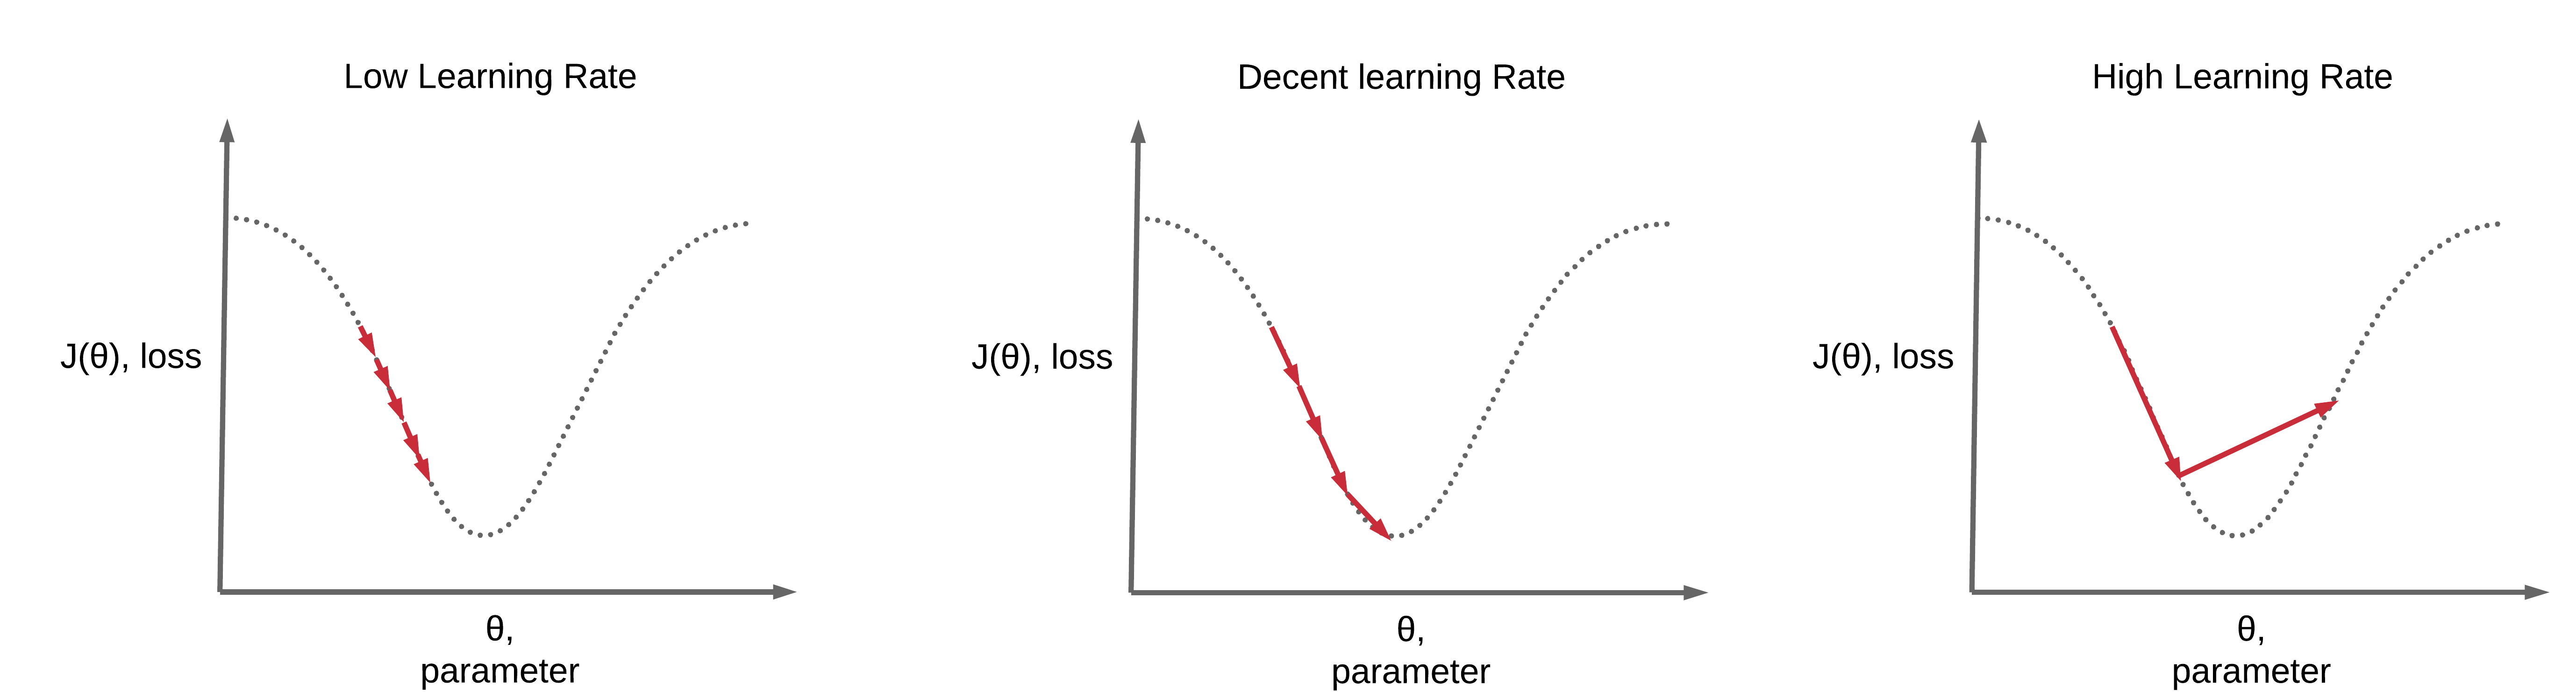
\includegraphics[width=1\textwidth]{pics/gradient.png}
\end{figure}

Dado el diseno de la red neuronal definido en el punto anterior, comenzamos con la declaracion del modelo con vistas a su entrenamiento, guardado, validacion y posterior uso.

%TODO: Reescribir
Es importante destacar que el entrenamiento de una IA tiene una gran parte de ensayo-error, por lo que en el codigo que veremos a continuacion, aunque los parametros son los utilizados en el entrenamiento final del modelo, para llegar a ellos han sido necesarios muchos intentos y modificar muchas variables junto con las comprobaciones posteriores pertinentes hasta llegar a ellos.

La declaracion del modelo y otros parametros necesarios, se definen a traves de la API de Tensorflow junto con Keras, que pone a nuestra disposicion numerosas utilidades de las cuales podemos informarnos a traves de su documentacion oficial. El código se muestra a continuación:

\noindent\begin{minipage}{\textwidth}
\begin{lstlisting}[language=python]
dataset_dir = pathlib.Path('instalation/data/Kanji_Images')  

batch_size = 32  
source_height = 64  
source_width = 64  

training_dataset = tf.keras.utils.image_dataset_from_directory(
    dataset_dir,  
    validation_split=0.2,  
    subset='training',  
    seed=39,  
    image_size=(source_height, source_width),  
    batch_size=batch_size)  

validation_dataset = tf.keras.utils.image_dataset_from_directory(
    dataset_dir,
    validation_split=0.2,
    subset='validation',
    seed=39,
    image_size=(source_height, source_width),
    batch_size=batch_size)
    
optimizer_model = keras.optimizers.Adam(learning_rate=0.0005)
loss_model = tf.keras.losses.SparseCategoricalCrossentropy(from_logits=True)
model.compile(optimizer=optimizer_model,
              loss=loss_model,
              metrics=['accuracy'])
epochs = 50 
training = model.fit(training_dataset,
                     validation_data=validation_dataset,
                     epochs=epochs)
model.save('trainings/fullmodel2.keras') 
\end{lstlisting}
\end{minipage}\\

En primer lugar, nos encargamos de crear las variables que contendran el directorio de nuestro dataset, el tamaño del batch, y el alto y ancho de las imagenes de nuestro dataset.

A continuacion, definimos los dataset de entrenamiento y validacion a traves de una de las herramientas ofrecidas por Keras, a las que le pasaremos el directorio, el porcentaje de separacion aleatoria entre dataset de entrenamiento y validacion, el nombre del subset, una semilla de aleatoriedad para evitar que la IA se acostumbre a determinados patrones, el tamano de nuestras imagenes y el tamano de nuestro batch.

Finalmente, inicializamos nuestras variables para el optimizador y nuestra funcion de perdida. El optimizador utilizado para este caso ha sido Adam, ya que tras numerosas pruebas, el entrenamiento mas correcto y eficiente en terminos computacionales era este. Lo utilizamos, como podemos ver en el codigo, con un learning rate de 0.0005. Nuestra funcion de perdida sera SparseCategoricalCrossentropy.

Con todas estas variables correctamente definidas, podemos realizar la compilacion de nuestro modelo pasandole las variables que acabamos de crear, definir un numero de epocas, y llamar a la funcion .fit(), que se encargara de hacer una iteración de entrenamiento por el numero de epocas especificado. En nuestro caso, ademas, asignamos el valor devuelto por esta funcion a una variable que nos sera util mas adelante en el codigo para consultar valores y generar graficos de los resultados obtenidos en el entrenamiento.

Finalmente, utilizamos la funcion .save() de nuestro modelo para que se genere un archivo en cuyo interior se almacenan los pesos del modelo entrenado, que podremos cargar mas tarde para realizar las predicciones necesarias.\\


Todos estos terminos tienen un fuerte componente matematico detras, que se extiende al objetivo de este documento, por lo que las explicaciones plasmadas aqui unicamente pretenden clarificar al lector acerca de los terminos utilizados y el papel que juegan en el desarrollo del proyecto. 

Para mas informacion respecto tanto al contexto matematico como a las diferentes definiciones y usos de las herramientas mencionadas en esta sección, pueden consultarse las fuentes que figuran en el anexo de informacion adicional externa:\\


\subsubsection{Validacion}
Con cada época del entrenamiento, es convencion en desarrollo de IA realizar una validacion de este, para ver que progresa como es debido y los resultados avanzan en la direccion adecuada, hasta llegar a una validacion con la que estemos satisfechos que nos indique que el modelo que hemos entrenado esta listo para su uso. En este punto debemos desarrollar una herramienta que compruebe tanto con datos del dataset, como externos a el, que las predicciones que realiza de los datos que le pasamos son acertadas con suficiente certeza y el suficiente numero de veces.

Es importante realizar un batch de validación porque entrenar una IA y validar con el mismo set de datos con la que la hemos entrenado no es recomendable; en primer lugar, no sabemos si es capaz de reconocer datos que le sean desconocidos, y en segundo lugar, las métricas que recibamos sobre la precision y la tasa de acierto se verán afectadas precisamente por haberse entrenado con los mismos datos que intentamos predecir.

La idea detras de este desarrollo es poder obtener informacion precisa sobre el rendimiento de nuestra IA, de forma que podamos ajustar sus parametros en base a ensayo-error (practica muy comun en entrenamiento de IAs) hasta dar con unos ajustes cuyo rendimiento sea satisfactorio. Esto nos permitira entrenar un numero considerable de épocas, hasta que los resultados de la validación muestren un estancamiento del ratio acierto/error. 

Cabe mencionar que es en este punto donde debemos dejar de entrenar la IA, ya que forzarla a continuar un numero excesivo de épocas para conseguir mejoras marginales, puede generar el llamado \hyperref[sec:terms]{\textit{overfitting}\tec}, que causara un mayor numero de falsos resultados a la hora de trabajar con datos ajenos al dataset original.


\subsection{Implementacion}

En esencia, debemos encargarnos de que nuestra IA pueda ser utilizada accediendo a ella sin necesidad de ejecutar manualmente un script (como hacemos con nuestra validacion), y que los datos que esta genera, puedan ser recibidos e interpretados por otras herramientas en lugar de ser impresos en una consola. Para ello, se distinguen dos puntos fundamentales que desarrollamos a continuación.

Para conocer en detalle el funcionamiento interno, casos de uso de la aplicación, etc. se incluyen varios diagramas UML disponibles en el \hyperref[sec:uml]{\textit{Anexo 2.}}

\subsubsection{Configuración de los metodos}
Siguiendo la documentacion oficial de la libreria que utilicemos, debemos definir los parametros que la API desea recibir, el protocolo utilizado, la ruta donde desea recibirlos, y demas configuraciones necesarias para despues poder consumir esa funcionalidad a traves de protocolo HTTP, ya sea utilizando \hyperref[sec:terms]{\textit{Postman}\tec} o un navegador.

En este caso, tras todo el desarrollo de la IA, se hace una busqueda sobre las librerias con las que podemos proceder a crear la API. Se dedcide utilizar las librerias de FastAPI y Uvicorn. La primera libreria se encargará de permitirnos crear las funcionalidades que necesitemos para interactuar con nuestro codigo. La segunda se trata de una implementacion para Python de un servidor web ASGI, lo que nos permitira acceder a el a través de una red.

Una vez configurada la API y levantado el web service con uvicorn, comprobamos que todos estos metodos y la configuracion del servicio funcionen correctamente, intentando realizar una request a traves de Postman. Una vez consigamos que la respuesta HTTP devuelta sea satisfactoria, aunque no tengamos nuestro resultado, confirmaremos que la configuracion de estos puntos es la correcta, y necesitara poca o ninguna configuracion extra de aqui en adelante.

\subsubsection{Presentación del resultado}
Una vez desarrollada correctamente la configuracion de la API, faltaría la parte del desarrollo en la que los datos que hemos enviado a nuestro servidor se procesan y recibamos una respuesta en el formato correcto con los datos que ha generado nuestra IA.

Sera trabajo de otras herramientas utilizadas como procesar la informacion enviada por nuestra API, sin embargo el formato en el que esta envie los datos debe ser algo legible y facilmente procesable, por lo que nuestro resultado se configura para que devuelva un JSON formateado de forma especifica para su posterior lectura.

\noindent\begin{minipage}{\textwidth}
\begin{lstlisting}[title=Formato del JSON de respuesta., numbers=none]
    {
      "result": [
        {
        "character": "kanji1",
        "certainty": "0.5"
        },
[...]
        {
        "character": "kanji5",
        "certainty": "0.04"
        }
      ]
    }
\end{lstlisting}
\end{minipage}

\subsection{Alojamiento}
Uno de los objetivos de este proyecto es poder consumir la IA a traves de un WebService expuesto a internet, por lo que uno de los pasos a seguir sera configurar un servidor privado donde alojar la API y exponer sus funcionalidades a internet. Para realizar este punto, debemos seguir los siguentes pasos:

\subsubsection{Montaje e instalacion del servidor}
Se plantea usar como servidor una torre de bajo presupuesto. En este ordenador se instalara la version estable mas reciente de \hyperref[sec:terms]{\textit{Linux Debian}\tec}, sin ningun tipo de interfaz grafica ni utilidades extras a las propias del Sistema Operativo a parte de Docker, para la creacion de \hyperref[sec:terms]{\textit{containers}\tec}; Git, para descarga y manejo de repositorios; y NeoVim, un editor de texto de terminal para gestionar los archivos de configuracion necesarios en el servidor

La instalacion y configuracion inicial se realiza de la forma habitual, y una vez configurada la red y el acceso por \hyperref[sec:terms]{\textit{SSH}\tec}, desconectamos todos los perifericos y utilizamos una conexion SSH para acceder a el sin necesidad de compartir o utilizar perifericos extra, conectandonos desde el mismo sistema desde el que realizamos nuestro desarrollo.

Esto es particularmente util ya que quitamos del servidor cualquier tipo de software que pueda consumir sus recursos de forma innecesaria. En su lugar, trabajamos con el mismo equipo con el que desarrollamos y configuramos todas las caracteristicas propias del codigo fuente, y a traves de una consola de comandos, modificamos y configuramos aquello que necesitemos en nuestro servidor de forma remota.

\subsubsection{Networking}
Para que el sistema que instalamos en el punto anterior pueda realizar las funciones de servidor que necesitamos, tenemos que realizar diversos ajustes de \hyperref[sec:terms]{\textit{networking}\tec} que explicamos a continuación.\\

En primer lugar, debemos asegurarnos una \hyperref[sec:terms]{\textit{IP publica}\tec}. Para esto, se contacta con nuestro \hyperref[sec:terms]{\textit{ISP}\tec}, y se le solicita que se nos asigne una \hyperref[sec:terms]{\textit{IP dinamica}\tec} fuera del \hyperref[sec:terms]{\textit{CGNAT}\tec}.

Hecho esto, le asignamos a nuestro servidor una \hyperref[sec:terms]{\textit{IP estatica}\tec} dentro de nuestra red local, y la asignamos a un \hyperref[sec:terms]{\textit{dominio}\tec} de tal forma que las conexiones del exterior siempre accedan a través de la misma dirección.

Legalmente, nuestro ISP tiene la obligacion de proveernos una IP publica, sacandonos del CGNAT en el que nos tengan. Por suerte, O2 (Telefonica) unicamente asigna IPs publicas a sus clientes, por lo que durante este desarrollo no se ha necesitado llevar a cabo este trámite.

Técnicamente, también tienen la obligacion de proveernos una IP estatica, sin embargo, al contrario que una IP dinamica como mencionamos anteriormente, esto no se contempla de forma gratuita, sino que se trata de un servicio de pago.

Dado que para este proyecto ya disponemos de una IP publica, nos es suficiente para poder configurar el servidor acorde a nuestras necesidades. En primer lugar, se compra un dominio a traves de Namecheap.com (otterleek.com). A continuacion, nos registramos en NoIP.com, un servicio gratuito que se encarga de monitorizar nuestra IP y asignarle de forma dinamica un \hyperref[sec:terms]{\textit{DNS}\tec} desde el que poder conectarte.

En terminos generales, la IP publica que nos proporciona nuestro ISP se mantiene hasta que nuestro router se reinicia o pierde su conexion. Si en algún momento el ISP cambia nuestra IP, NoIP.com lo detecta, y apunta el dominio que hemos solicitado a nuestra nueva IP. NoIP ofrece este servicio de forma gratuita con la condicion de confirmar una vez al mes que continuamos utilizando sus servicios.

Solucionado el problema de que podamos acceder a nuestra IP en cualquier momento que queramos independientemente de si ha cambiado o no, quedaria reasignar nuestro dominio al que hemos adquirido. Para ello la propia pagina de Namecheap tiene unas opciones de configuracion DNS con las que podremos realizar estos cambios. Para nuestra IA crearemos un subdominio al que podremos enviar una petición HTTP (kanji.otterleek.com) que apuntaremos al DNS facilitado por NoIP.

Con esta configuracion ya tendriamos el networking listo para poder configurar un container a través del que podremos hacer consultas sobre nuestro web service.

\subsubsection{Dockerizacion}
Por ultimo, dentro de nuestro servidor, para que pueda convivir con mas aplicaciones y herramientas, instalaremos nuestra API en un container de Docker y le asignaremos el puerto que deseemos, asegurandonos de que todo esta correctamente expuesto a internet y que el container es capaz de mantenerse activo sin mantenimientos adicionales.

\noindent El proceso para esto es bastante simple. En nuestro directorio root del servidor, introducimos los comandos

\noindent\begin{minipage}{\textwidth}
\begin{lstlisting}[numbers=none]
mkdir -p Docker/Kanji-AI && cd $_
nvim Dockerfile
\end{lstlisting}
\end{minipage}
Esto creara un directorio donde almacenaremos toda la configuracion de nuestro container y un archivo Dockerfile donde definiremos los parametros de instalacion e inicializacion del container:

\noindent\begin{minipage}{\textwidth}
\begin{lstlisting}[numbers=none]
FROM python:3.8
WORKDIR /code
COPY ./requirements.txt /code/requirements.txt
RUN pip install --no-cache-dir --upgrade -r /code/requirements.txt
COPY ./app /code/app
CMD ["uvicorn", "app.main:app", "--proxy-headers", "--host", "0.0.0.0", "--port", "39000"]
\end{lstlisting}
\end{minipage}
Para que el proyecto funcione correctamente debera instalar una serie de librerias que le pasamos en un archivo de texto llamado \textit{requirements.txt} como puede verse en el fichero anterior, que debemos crear con el siguiente contenido:

\noindent\begin{minipage}{\textwidth}
\begin{lstlisting}[numbers=none]
fastapi>=0.68.0
pydantic>=1.8.0
uvicorn>=0.15.0
numpy
tensorflow
pillow
python-multipart
matplotlib
\end{lstlisting}
\end{minipage}

Este proceso creara una instalacion del container con las dependencias necesarias, sin embargo, necesitamos configurarlo correctamente para que al levantarse, se conecte correctmente con los puertos indicados, en la network adecuada, y a traves del protocolo HTTPS.

Para esto debemos crear un \textit{docker-compose.yml}, aunque antes debemos realizar una correcta instalacion y configuracion de Traefik, un \hyperref[sec:terms]{\textit{reverse-proxy}\tec} y \hyperref[sec:terms]{\textit{load-balancer}\tec} integrado nativamente con Docker para permitirnos exponer a internet servicios desde nuestros containers. Como la configuracion de Traefik es compleja y extensa, y va mas alla del objetivo de esta documentacion, estara disponible una breve explicacion en el \hyperref[sec:Traefik]{\textit{Anexo 3}} sobre configuracion de Traefik.

Una vez realicemos la correcta instalacion y configuracion de Traefik, podremos crear el fichero mencionado anteriormente con el siguiente contenido:

\noindent\begin{minipage}{\textwidth}
\begin{lstlisting}[numbers=none]
name: kanjiAI
services:
    kanjiAI:
        build: .
        image: kanji-AI
        container_name: kanji-AI
        working_dir: /code/app
        command: "uvicorn main:app --host 0.0.0.0 --port 39000 --reload"
        ports:
            - "39000:39000"
        volumes:
            - .app:/code/app
        restart: "unless-stopped"
        networks:
            - traefik-global-proxy
        labels:
            - "traefik.enable=true"
            - "traefik.http.routers.ai.rule=Host(`kanji.otterleek.com`)"
            - "traefik.http.routers.ai.tls.certresolver=letsencrypt"
            - "traefik.http.routers.ai.entrypoints=https"
            - "traefik.http.services.ai-service.loadbalancer.server.port=39000"
networks:
    traefik-global-proxy:
        external: true
        
\end{lstlisting}
\end{minipage}

Tras realizar esta configuracion, debemos abrir el puerto 39000 TPC en nuestro router. Podemos hacer esto accediendo a él a traves de nuestra puerta de enlace y utilizando el software que los propios router implementan.

Por último, debemos incluir nuestro desarrollo en una carpeta llamada \textit{app/} (como puede verse en los archivos de configuracion) dentro de nuestra carpeta de configuraciones del container, y levantar el container en modo detached para que el proceso del container no inutilice nuestra consola.

\noindent\begin{minipage}{\textwidth}
\begin{lstlisting}[numbers=none]
docker compose up -d
\end{lstlisting}
\end{minipage}
Nuestra IA estaria en este punto lista para utilizarse a traves de internet, y podemos comprobar su correcto funcionamiento haciendo una peticion HTTP \hyperref[sec:terms]{\textit{multipart}\tec} al dominio mencionado anteriormente (https://kanji.otterleek.com) con una imagen adjunta. La imagen llegara entonces a nuestro WebService y nuestro desarrollo realizara una prediccion de los cinco kanjis mas posibles en esa imagen, devolviendonos una respuesta HTTP en el formato JSON mencionado previamente en esta misma sección.

\subsection{Creacion de la interfaz}

Respecto a la creacion de la interfaz, simplemente distinguiremos dos desarrollos al respecto, el diseno de la interfaz incluyendo sus funcionalidades, disposicion y la interaccion entre sus ventanas por un lado, y el desarrollo para contactar con el web service y procesar sus respuestas por otro.

\subsubsection{Front end}
La intencion original es que la app sea extremadamente simple, disponiendo de dos funcionalidades basicas, capturar una imagen (únicamente para dispositivos con cámara), y cargar una imagen desde la memoria del dispositivo.

Una vez cargada, mostrar la imagen a enviar para asegurarnos de que se ve correctamente y el caracter esta correctamente acotado en la imagen para solicitar su prediccion, junto con dos botones, uno para eliminar la imagen seleccionada y repetir el proceso, y otra para contactar con el web service, que una vez pulsada, esperara la respuesta de este, y nos llevara a una tercera ventana donde se muestre la prediccion junto con el boton de salida.

\begin{comment}
Para todo este proceso, tanto la explicacion del codigo como de la ejecucion son demasiado especificos y aportan demasiado poco a la memoria del proyecto, por lo que considero que lo unico a explicar en este apartado es que hemos decidido utilizar Flutter, un framework de Dart para diseno de aplicaciones multiplataforma que permite reutilizar nuestro codigo con minimas modificaciones para crear apliacaciones en diferentes sistemas y plataformas.
end{comment}
Para todo este desarrollo hemos utilizado Flutter, un framework basado en el lenguaje Dart enfocado en el desarrollo de aplicaciones multiplataforma que permite reutilizar nuestro código con las modificaciones mínimas para crear versiones para los dispositivos mas utilizados hoy en día.

El desarrollo de la interfaz es una simple estructura de componentes, por lo que no considero necesario entrar en detalle sobre el código como tal, que estará disponible en el repositorio. Para cualquier información relativa a esta parte del desarrollo, puede consultarse la documentacion oficial de Flutter.

\subsubsection{Back end}
Respecto a la funcionalidad que se desarrolle por debajo de la interfaz, nos centraremos casi de forma exclusiva en poder enviar la imagen al web service correctamente, y ser capaces de recibir y procesar su respuesta para mostrarla por pantalla.

Hay diversas utilidades para hacer que el dispositivo cargue una imagen de la galeria o acceda a la camara para capturar una imagen, por lo que no nos vamos a detener en la explicacion de esto, sin embargo, la parte compleja de este desarrollo consiste en realizar satisfactoriamente una petición HTTP multipart que nos permita enviar la imagen a nuesto WebService, y recibir y formatear su respuesta correctamente.

Esta parte del desarrollo se sustenta sobre dos fragmentos de código que explico a continuación.

Flutter implementa nativamente el envio de peticiones HTTP multipart, por lo que hemos utilizado la siguiente funcion para solicitar una prediccion a nuestra IA:

\noindent\begin{minipage}{\textwidth}
\begin{lstlisting}[language=java]
Future<Prediction> requestPredictionAPI(File kanji, BuildContext context) async{
    final request = http.MultipartRequest('POST', Uri.parse('https://kanji.otterleek.com/'));
    request.files.add(await http.MultipartFile.fromPath('file', path!));
    final response = await request.send();
    if (response.statusCode==200){
        String b = (await http.Response.fromStream(response)).body;
        return Prediction.fromJson(jsonDecode(b));
    }
    else{
        Navigator.of(context).push(MaterialPageRoute(builder: (context) => Unavailable())); 
        throw Exception('Kanji AI Predict WebService is unavailable');
    }
}
\end{lstlisting}
\end{minipage}
\newpage
Donde Prediction es una clase que recoge la respuesta HTTP y la transforma en consecuencia para poder acceder a los datos de respuesta desde el codigo mas adelante:

\noindent\begin{minipage}{\textwidth}
\begin{lstlisting}[language=java]
class Prediction{
    final List<Content> content;
    Prediction({
        required this.content,
    });
    factory Prediction.fromJson(Map<String, dynamic> json) => Prediction(
        content: List<Content>.from(json['result'].map((x) => Content.fromJson(x))));
    Map<String, dynamic> toJson() => {
        "result": List<dynamic>.from(content.map((e) => e.toJson()))
  };
}

class Content {
    final String character;
    final double certainty;
    Content({
        required this.character,
        required this.certainty
    });
    factory Content.fromJson(Map<String, dynamic> json) => Content(character: json['character'], certainty: json['confidence']);
  
    Map<String, dynamic> toJson() => {
        "character": character,
        "certainty": certainty
    };
}
\end{lstlisting}
\end{minipage}




%%%%%%%%%%%%%%%%%%%% PUNTOS DE MEJORA %%%%%%%%%%%%%%%%%%%%%%%
\newpage

\section{Puntos a mejorar}
\label{sec:Improvements}

Aunque la realizacion de este proyecto es satisfactoria, debido a la falta de tiempo, capacidades, u otras variables, algunos aspectos de este proyecto tienen una amplia capacidad de mejora. En este punto trataremos brevemente futuras mejoras a desarrollar para nuevas versiones. Mencionar antes de nada, que el objetivo de este apartado no es presentar aspectos con los que ampliar la funcionalidad de la aplicacion, sino para elaborar puntos de mejora en el rendimiento, la facilidad de uso, etc. considerables que no se han podido aplicar por diversas circunstancias.

\begin{itemize}
    \item \textbf{Utilizar \hyperref[sec:terms]{\textit{data augmentation}\tec}}: El uso de data augmentation puede mejorar mucho la capacidad predictiva de la IA en casi cualquier escenario, sin embargo, no se ha implementado porque para esto se requiere de un poder computacional y un tiempo de entrenamiento muy elevado.
    \item \textbf{Implementar distinción de kanjis}: Se podría implementar un algoritmo capaz de analizar la imagen e identificar kanji que pueda haber en ella, y generar un encuadre correcto en torno a la figura para el posterior análisis por parte de nuestra IA. Esto haría que la experiencia de usuario y los casos de uso mejorasen drásticamente, sin embargo no se ha considerado su implementacion tanto por el factor de tiempo como por el de dificultad.
    \begin{comment}
    Realizar segmentacion en las imagenes haria que no fuese necesario cuadrar en el centro de la imagen un kanji y asegurarnos de que esta lo mas aislado posible de otros elementos. Esta condicion es una de las que mas entorpecen el funcionamiento y la experiencia de esta herramienta, por lo que es un punto a considerar muy importante, sin embargo no se ha implementado por la dificultad que supondria la generacion del algoritmo necesario para reconocer la parte necesaria y reformatear la imagen en consecuencia.
    end{comment}
    \item \textbf{Mejorar el procesado de imagenes}: La IA es propensa a fallos cuando las fotografias se realizan en escenarios de poca luz debido al poco rango dinamico de los dispositivos, la cantidad de ruido, y el poco contraste presente en las imagenes tomadas en estas circunstancias. Un procesamiento de la imagen mas exhaustivo, que analice la cantidad de luz, el contraste de la escena, y sea capaz de proveer un kanji en el mayor numero de condiciones desfavorables posibles es un aspecto importante a tener en cuenta. 
    \item \textbf{Interfaz mas profesional}: El mayor peso de este proyecto recaia sobre todo el proceso de creacion de la IA y la comunicacion con ella, por lo que la interfaz de usuario es excesivamente simple y con muy pocas funcionalidades. Es necesario considerar cambiar este diseno para sus futuras versiones y a ser posible anadir alguna funcionalidad extra para la comodidad del propio usuario.
    \item \textbf{Crear un instalador}: Se contempla como uno de los futuros desarrollos, una forma de crear un instalador de esta IA de forma que se aloje localmente en un dispositivo y podamos acceder a ella a traves de una conexion local sin necesidad de acceder a internet.
\end{itemize}

%%%%%%%%%%%%%%%%%%%% RECURSOS HUMANOS %%%%%%%%%%%%%%%%%%%%%%%


\section{Recursos humanos}
\label{sec:HumanRes}

Los recursos humanos del proyecto son virtualmente inexistentes. El proyecto se desarrolla de forma unipersonal, gestionando mi tiempo y mis recursos para la conclusion de los objetivos marcados en este proyecto. 

Unicamente cabe destacar la ayuda puntual de companeros de clase, de profesion, y personal docente del centro que se vera reflejada en el anexo de agradecimientos.



%%%%%%%%%%%%%%%%%%%% RECURSOS MATERIALES %%%%%%%%%%%%%%%%%%%%%%%

\newpage
\section{Recursos materiales}
\label{sec:Resources}

\noindent El detalle de todos los recursos materiales utilizados en este proyecto consiste en:
\subsection{Hardware}
\begin{itemize}
    \item Un smartphone donde realizar pruebas de la aplicacion movil
    \item Un ordenador donde se desarrollara el proyecto junto con sus perifericos compuesto por:
    \begin{itemize}
        \item CPU AMD Ryzen5 5600 
        \item GPU AMD Radeon 6600 
        \item RAM Viper 32Gb DDR4 
        \item SSD M.2 500Gb Crucial
        \item Otros componentes (PSU, Fuente de Alimentacion, Caja...)
        \item Teclado Logitech MX Keys
        \item Raton Logitech MX Master M3s
        \item Monitores AOC 24G2U (x2)
    \end{itemize}
    \item Un servidor compuesto por:
    \begin{itemize}
        \item CPU Intel i3 2120
        \item RAM Kingston 6Gb DDR
        \item SSD SATA3 Kingston 160Gb
        \item Otros componentes (PSU, Fuente de Alimentacion, Caja...)
    \end{itemize}
    \item Diversos cables de conexion, corriente, etc. (Ethernet, HDMI, DP, USB-C...)
\end{itemize}

\subsection{Software y Servicios}
\begin{itemize}
    \item Un dominio ("otterleek.com")
    \item Una conexion a Internet (O2)
    \item Licencias:
    \begin{itemize}
        \item PyCharm Community Edition
        \item Debian 12.2
        \item Docker
        \item Visual Studio Code
        \item Postman
        \item Overleaf
    \end{itemize}
    \item Diversas librerias de terceros (Tensorflow, Keras, Pillow...) que han sido mencionadas a lo largo del proyecto
\end{itemize}
\newpage

\subsection{Presupuesto}

El total del presupuesto incluye los 5 meses de desarrollo de la aplicacion, y un solo ano de dominio, sin embargo con futuros desarrollos, debido al pago de estos servicios, puede verse incrementado.

*Algunos componentes son piezas genericas de fabricantes que no estan disponibles al publico para su compra, por lo que ha sido todo agrupado bajo un mismo nombre generico, y su precio se ha calculado en base a precios de componentes de caracteristicas similares, al igual que con los cables utilizados, muchos proveidos por los propios fabricantes de los componentes. Estos elementos son: Caja, placa base y fuente de alimentacion del servidor, pilas CMOS, pasta termica, cables SATA, cables HDMI, cables DisplayPort, cables USB y USB-C y cables de alimentacion.\\
    
\begin{center}
    
\begin{tabularx}{\linewidth}{
| >{\raggedright\arraybackslash}X
 >{\raggedleft\arraybackslash}X
 >{\raggedleft\arraybackslash}X | 
}
\toprule
Detalle                     &    Cantidad           &  Precio\\
\midrule

Asus Prime b550-Plus        &    x1 ud.             &  109.99\euro\\
AMD Ryzen5 5600             &    x1 ud.             &  137.52\euro\\
Intel i3 2120               &    x1 ud.             &  32.46\euro\\
Xilence XC032               &    x1 ud.             &  16.01\euro\\
XFX Speedster SWFT 210      &    x1 ud.             &  229.90\euro\\
Viper 16Gb DDR4 3600mHz     &    x2 ud.             &  36.59\euro\\
Kingston 4Gb DDR3 1333mHz   &    x1 ud.             &  22.14\euro\\
Kingston 2Gb DDR3 1333mHz   &    x1 ud.             &  17.24\euro\\
M.2 Crucial 500Gb           &    x1 ud.             &  40.99\euro\\
SATA3 Kingston 160Gb        &    x1 ud.             &  21.80\euro\\
SeaSonic Core GM 500W       &    x1 ud.             &  86.99\euro\\
Lian Li Mesh 205            &    x1 ud.             &  61.72\euro\\
AOC 24G2U                   &    x2 ud.             &  255.10\euro\\
Logitech MX Keys            &    x1 ud.             &  89.99\euro\\
Logitech MX Mastwer M3      &    x1 ud.             &  91.41\euro\\
Xiaomi Redmi Note 12 Pro 5G &    x1 ud.             &  289.99\euro\\
Otros componentes*          &    sin especificar    &  97.39\euro\\
Diversos cables*            &    sin especificar    &  34.02\euro\\
Dominio "otterleek.com"     &    pago anual (x1)    &  9.76\euro\\
Conexion a internet         &    pago mensual (x5)  &  38.00\euro\\

\bottomrule
\textsc{\textbf{TOTAL}} & & \fbox{\textbf{2002.11\euro}}\\
\bottomrule
\end{tabularx}
\end{center}


\newpage


%%%%%%%%%%%%%%%%%%%% ANEXOS %%%%%%%%%%%%%%%%%%%%%%%

\section{Anexos}

\subsection{Terminos tecnicos}
\label{sec:terms}
\begin{itemize}
    \item \textbf{Kanji:} Son sinogramas utilizados en la escritura del idioma japones, junto con los lisabarios \textit{hiragana y katakana}. Se usan mayoritariamente para expresar conceptos, a diferencia de su variante china, donde se emplean tambien con caracter fonetico. Asimismo, existen combinaciones de kanji  que no obeceden a su significado original y modifican el valor fonetico asignado de sus componentes. A cada kanji le corresponde un significado y se usa como determinante la raiz de la palabra, y sus derivaciones o conjugaciones se expresan mediante el hiragana. Un kanji puede tener diferentes pronunciaciones o 'lecturas' dependiendo de su contexto, uso y localizacion, pero es muy poco comun que un kanji tenga varios significados que disten mucho entre ellos.
    \item \textbf{Modelo:} Consiste en un formato de datos en el que se especifican las instruccciones de procesamiento de datos para permitir que el sistema que éste define sea capaz de aprender patrones específicos presentes en los conjuntos de datos que tenemos como objetivo, y formar predicciones a partir de ellos.
    \item \textbf{Data science:} Se trata de una disciplina cientifica centrada en el analisis de grandes fuentes de datos para extraer informacion de ellas, comprender su significado y descubrir patrones dentro de ellas. En ella se combinan matematicas, estadistica  e informatica, generalmente con el objetivo de optimizar la toma de decisiones respecto a un problema concreto.
    \item \textbf{Unicode:} Es un estandar de codificacion de caracteres disenado para facilitar el tratamiento informatico, transmision y visualizacion de textos de numerosos idiomas y disciplinas. Se define cada caracter mediante un nombre e identificador numerico y todos se tratan de forma equivalente de forma que se puedan utilizar en un texto sin necesitad de utilizar marcas o caracteres de control. A dia de hoy, el sistema puede representar 149.186 caracteres, incluyendo entre ellos caracteres de formato como saltos de linea o tildes, de un espacio posible de 1.114.112(0x10FFFF) menos los caracteres reservados para el uso internno del sistema.
    \item \textbf{IA:} De Inteligencia Artificial. Es un campo de la ciencia relacionado con la creacion de sistemas que sean capaces de razonar, aprender y actuar simulando la inteligencia humana o involucrando cantidades de datos mas alla de la capacidad de analisis humana. Es un campo que en si mismo abarca muchas disciplinas, como la informatica, el analisis de datos, la estadistica, el procesamiento del lenguaje natural, la neurociencia, entre otras. A nivel practico, se trata de una tecnologia basada en el aprendizaje automatico, que analiza datos y genera las respuestas requeridas frente a un problema.
    \item \textbf{API:} Del ingles, Application Programming Interface, es un codigo o conjunto de estos que permiten a diferentes aplicaciones comunicarse entre si y compartir informacion y funcionalidades a modo de intermediario entre ambos sistemas.
    \item \textbf{Web service:} Es una forma estandarizada de establecer una comunicacion y/o realizar intercambios de datos entre diferentes aplicaciones a través de internet a través de los protocolos comunmente utilizados en tecnologías web.
    \item \textbf{Clasificador KNN:} Del ingles, K-Nearest-Neighbors, es un metodo de clasificacion que busca en las observaciones mas cercanas al dato de entrada, y lo clasifica basandose en la mayoria de datos que le rodean. Se trata de un algoritmo supervisado y basado en instancia, es decir, que nuestros datos estan etiquetados con una clase o resultado, y el algoritmo predice en base a estos (supervisado) y que el algoritmo no realiza un aprendizaje como tal, sino que carga las instancias en memoria para realizar la prediccion en base a estas.
    \item \textbf{Red neuronal:} En terminos simples, es un metodo de IA que se encarga de procesar datos de una manera inspirada en el funcionamiento de las neuronas del cerebro humano. Es un proceso que utiliza nodos interconectados en una estructura de capas capaz de producir un sistema adaptable que aprende en base a los errores producidos en sus procesos anteriores.
    \item \textbf{Validacion:} Se trata de un proceso por el cual analizamos la validez del modelo generado en base a la precision de sus predicciones. Para ello se utiliza un conjunto de validacion, que a diferencia de nuestro conjunto de datos principal, no se utiliza para ajustar los parametros del modelo, sino para evaluar su rendimiento final, y que no esta autocontenido en el conjunto de entrenamiento para producir resultados fiables.
    \item \textbf{OCR:} Del ingles Optical Character Recognition, es un metodo de reconocimiento de caracteres que es capaz de identificar y extraer textos a partir de una imagen.
    \item \textbf{Overfitting:} Es un efecto comun en el entrenamiento de IAs en el que nuestro modelo solo se ajusta a aprender los casos concretos que le estamos proporcionando durante el entrenamiento, y su rendimiento al reconocer nuevos datos de entrada se ve deteriorado. 
    \item \textbf{Postman:} Se trata de un cliente HTTP para producir, probar y utilizar APIs tipo REST a traves de peticiones HTTP con una interfaz grafica de usuario.
    \item \textbf{ASGI:} Del ingles Asynchronous Server Gateway Interface, es una interfaz estandar de comunicacion entre servidores web y aplicaciones web para manejar llamadas tanto sincronas como asincronas a traves de frameworks y aplicaciones de Python.
    \item \textbf{Linux Debian:} Se trata de una distribucion de GNU/Linux de codigo abierto, no comercial y totalmente gratuito para todos sus usos. Es una de las distribuciones mas importantes y populares hoy en dia en lo que respecta a la administracion de servidores por su alta estabilidad.
    \item \textbf{SSH:} Del ingles Secure Shell, es un protocolo de administracion remota tipo cliente-servidor a traves del cual los usuarios pueden tanto modificar como controlar servidores remotos a traves de una red bajo una capa de encriptacion.
    \item \textbf{Networking:} Se refiere a la creacion, configuracion y mantenimiento de redes a traves de las cuales multiples dispositivos y sistemas se comunican entre ellas y comparten informacion.
    \item \textbf{ISP:} Del ingles Internet Service Provider, hace referencia a la empresa encargada de proveer y gestionar nuestra conextion a internet.
    \item \textbf{IP:} Del ingles Internet Protocol, es una etiqueta numerica que identifica de manera logica y jerarquica a una interfaz (generalmente un dispositivo fisico) conectada a la red que utilice el protocolo de internet TCP/IP. Una IP Publica es por tanto, una direccion IP asignada por nuestro ISP a traves de la cual nos identificamos en internet al conectarnos. 
    Una IP dinamica se refiere al hecho de que, debido a la forma de trabajar de los ISP y el numero limitado de direcciones, la direccion IP puede verse afectada y cambiar en el tiempo (normalmente al reiniciar el router). Dentro de nuestra direccion de IP publica, existen un cierto numero de direcciones utilizables que llamaremos IPs internas. Estas direcciones suelen asignarse a distintos dispositivos de forma dinamica cuando acceden a una red local, sin embargo en la mayoria de los casos, podemos forzar a nuestros dispositivos a que se les asigne una IP interna concreta o estatica, para asegurarnos que siempre trabajan bajo la misma direccion.
    \item \textbf{CGNAT:} Se trata de una solución que utilizan algunos operadores para poder conectar varios equipos a internet bajo una misma dirección IP pública, a la que se asocian distintas direcciones IP privadas, por lo que todas éstas, pasan a ser identificadas bajo la misma dirección. Es por esto, que cuando un dispositivo fuera de la CGNAT intenta acceder a un dispositivo dentro de ella, en realidad esta intentando acceder a una dirección que contiene multiples destinos, y por tanto, hace inviable exponer direcciones a internet de forma pública.
    \item \textbf{Dominio:} Se trata de un nombre exclusivo que se le da a un sitio web para identificarlo y facilitar su acceso para los usuarios.
    \item \textbf{Container:} Son una forma de virtualizacion de sistemas operativos que contienen los ejecutables, librerías, y archivos de configuración necesarios para ejecutar algun tipo de servicio. Al contrario que con las maquinas virtuales, los containers no virtualizan abstrayendo el hardware de la maquina, sino que abstraen el sistema operativo al nivel mas bajo posible para que nuestro servicio o aplicacion pueda ejecutarse, por lo que son mucho mas ligeros y eficientes. La herramienta mas extendida para la gestión de containers a día de hoy es Docker.
    \item \textbf{Reverse proxy:} Se trata de un servidor que se situa delante de los servidores web, en una capa situada entre internet y el lado servidor y reenvia las solicitudes por parte del lado del cliente a dichos servidores. Suelen implementarse para aumentar la seguridad y el rendimiento de estos servicios.
    \item \textbf{Load balancer:} Se trata de una tecnologia orientada a la optimizacion de cargas de trabajo para que un grupo de servidores pueda hacer frente de forma eficiente a picos de trafico, equilibrando la carga entre los distintos servidores para mantener su capacidad a un nivel optimo, de modo que sean menos propensos a interrupcioes o ralentizaciones.
\end{itemize}

\newpage
\subsection{Esquemas}
\label{sec:uml}


%\begin{itemize}
    %\item Diagrama UML: Casos de uso.
    \begin{center}
        \centering 
        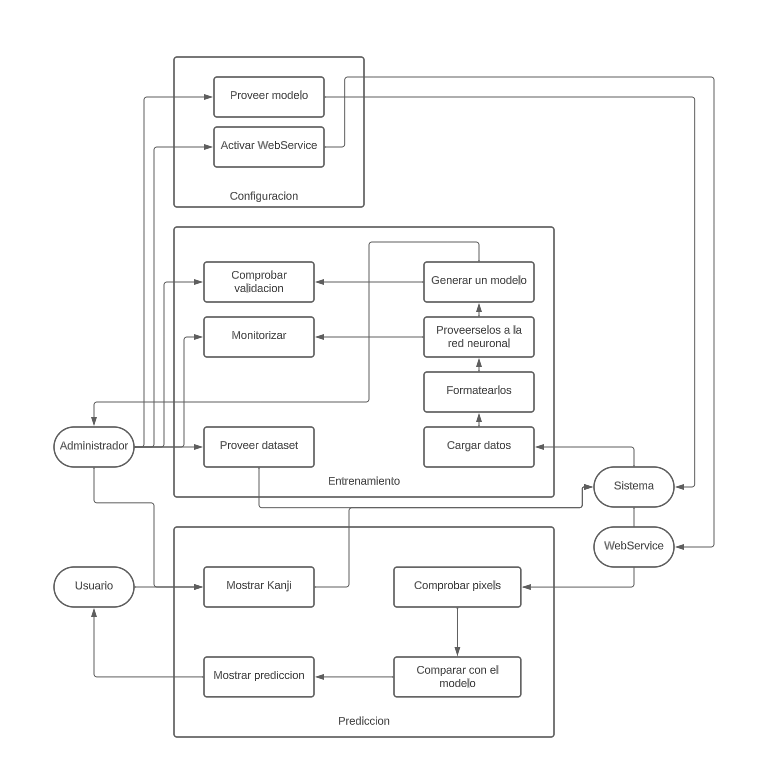
\includegraphics[width=1\textwidth]{pics/UseCases.png}
    \end{center}
   %\item Diagrama UML: Estado.
    \begin{center}
        \centering 
        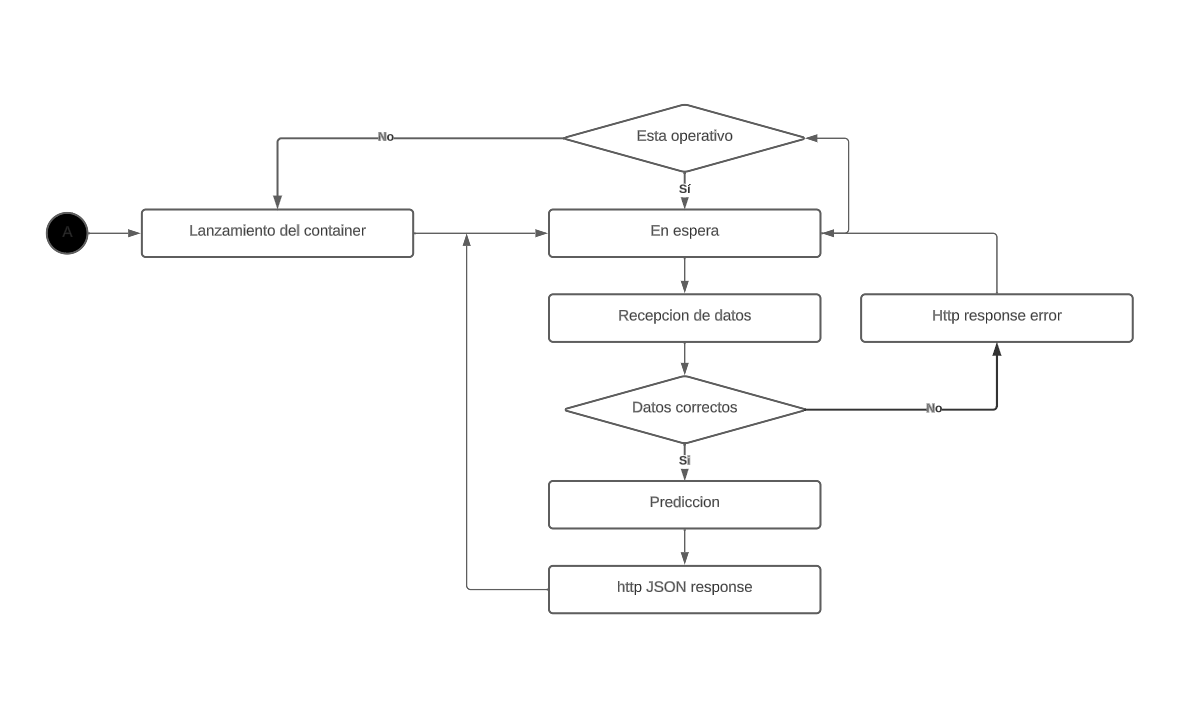
\includegraphics[width=1\textwidth]{pics/State.png}
    \end{center}
    %\item Diagrama UML: Despliegue.
    \begin{center}
        \centering 
        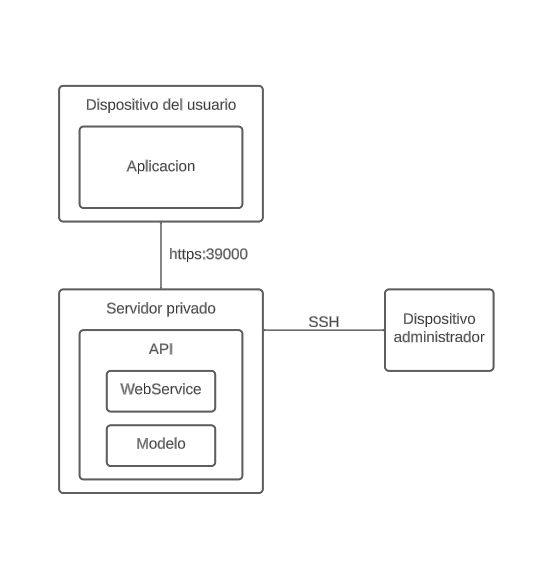
\includegraphics[width=0.7\textwidth]{pics/Deploy.png}
    \end{center}
    %\item Diagrama UML: Secuencia.
    \begin{center}
    \makebox[\textwidth]{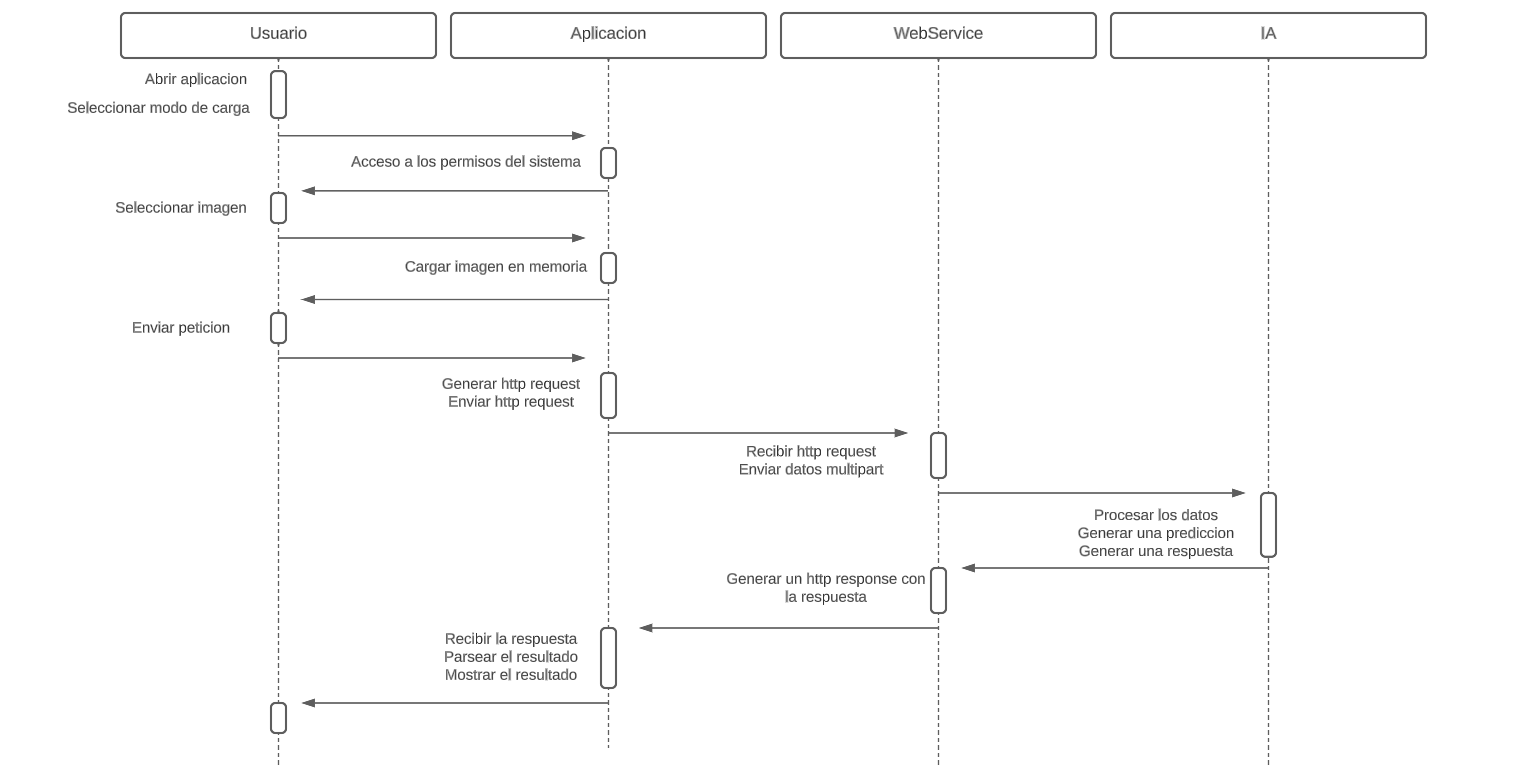
\includegraphics[width=\paperwidth]{pics/Sequence.png}}
    \end{center}
%\end{itemize}

\newpage
\subsection{Guia del desarrollador}
\label{sec:DevGuide}
\subsubsection{Configuracion de Traefik}
\label{sec:Traefik}
Como se ha explicado previamente, para poder exponer nuestra aplicacion a internet a traves de nuestro servidor dockerizado, debemos configurar correctamente Traefik.

Sin entrar en demasiados tecnicismos, en este punto desarrollaremos como crear una configuracion basica de Traefik con la que trabajar. Para mas informacion, Traefik dispone de una amplia documentacion online en la que solventar posibles dudas de funcionamiento y configuracion.

En primer lugar, debemos crear una carpeta para el container de docker dentro de nuestro servidor, que almacenara el servicio Traefik y su configuracion. En esta carpeta, crearemos un archivo \textit{docker-compose.yml} con la siguiente configuracion:

\noindent\begin{minipage}{\textwidth}
\begin{lstlisting}
version: "3.7"
services:
    traefik:
        image: traefik:2.4.8
        container_name: traefik
        networks:
            - traefik-global-proxy
        command:
            - --entrypoints.http.address=:80
            - --entrypoints.https.address=:443
            - --providers.docker=true
            - --providers.docker.network=traefik-global-proxy
            - --providers.docker.exposedByDefault=false
            - --api=true
            - --certificateresolvers.letsencrypt.acme.httpchallenge=true
            - --certificateresolvers.letsencrypt.acme.httpchallenge.entrypoint=http
            - --certificateresolvers.letsencrypt.acme.email=#<email>
            - --certificateresolvers.letsencrypt.acme.storage=/letsencrypt/acme.json
        labels:
            - traefik.enable=true
            - traefik.http.routers.to-https.rule=HostRegexp(`{host:.+}`)
            - traefik.http.routers.to-https.entrypoints=http
            - traefik.http.routers.to-https.middlewares=to-https
            - traefik.http.routers.traefik.rule=Host(`traefik.otterleek.com`)
            - traefik.http.routers.traefik.entrypoints=https
            - traefik.http.routers.traefik.middlewares=auth
            - traefik.http.routers.traefik.service=api@internal
            - traefik.http.routers.traefik.tls=true
            - traefik.http.routers.traefik.tls.certresolver=letsencrypt
            - traefik.https.middlewares.to-https.redirectscheme.scheme=https
            - traefik.https.middlewares.auth.basicauth.users=leek:#<KEY>
        ports:
            -80:80
            -443:443
        volumes:
            - ./data/letsencrypt: /letsencrypt
            - var/run/docker.sock:/var/run/docker.sock:ro
networks:
    traefik-global-proxy:
        name: "traefik-global-proxy" 
\end{lstlisting}
\end{minipage}\\

Con esta configuracion, y completando los puntos marcados con \#<...> con los parametros correspondientes, procederiamos a levantar el container, y a traves del docker compose y la configuracion ya mencionados en esta guia con la que levantamos nuestro web service, la ruta especificada en este ultimo ya entraria a traves del dominio y los puertos especificados y, ademas, a traves del protocolo https gracias a Let's Encrypt, una autoridad de certificacion gratuita y para uso publico.

De nuevo, como no es el propósito de este documento elaborar procesos de configuracion detallados respecto a las herramientas externas utilizadas en el proyecto, cualquier informacion adicional puede obtenerse en la documentación oficial de Traefik.\\

\subsubsection{.README}
\begin{lstlisting}

## Documentation

[Docker](https://linktodocumentation)
[Traefik](https://linktodocumentation)
[FastAPI](https://linktodocumentation)
[Python](https://linktodocumentation)
[Debian](https://linktodocumentation)
[Flutter](https://linktodocumentation)
[Tensorflow](https://linktodocumentation)

## Requirements

### For running:
 - Docker or Python 3.8 installed on your machine

### For training:
 - Python 3.8
 - 32Gb RAM as it is, adaptable to run on 16Gb
 - 2Gb of storage available
 - Recommended Ryzen 5 5600 or higher 
 * Note: Having a phisical GPU available will decrease significantly the training times. It is recommended to have CUDA, although we include a package in requirements.txt that allows a translation from AMD Technology to CUDA (only for Windows OS)

## Run locally

To train the IA locally: 

 - Clone the proyect
 - Install dependencies provided in `requirements.txt`
 - Download the dataset and the necessary fonts provided in the "necessary files" section
 - Unzip them in the root of the folder with the same name
 - Run the training_process.py script and wait for it to end


To run the IA locally without a container:

 - Clone the proyect
 - Install dependencies provided in `requirements.txt`
 - Run the main with uvicorn.


To deploy the IA locally end expose it to global network:

 - Follow the instructions provided in the section "Networking" of the documentation
 - Open the correct port
 - Clone the project
 - Create a container with the Dockerfile provided in the repository and the documentation
 - Run the container

 ## API Reference

#### Get a prediction

```https
  POST kanji.otterleek.ddns/
```

| Parameter | Type        | Description                |
| :-------- | :---------- | :------------------------- |
| `file`    | `multipart` | **Required**. Kanji image. |


\end{lstlisting}


\subsection{Agradecimientos}
\label{sec:Thanks}
Por ultimo, quiero dedicar este pequeño fragmento a agradecer a toda la gente que ha hecho este proyecto posible. En primer lugar, a Jordi Amoros por sugerirme la idea, introducirme en el campo de la inteligencia artificial, y ayudarme con la revision tanto del proyecto, como de esta documentación. En segundo lugar, a Vadim 'Ame' Perepelitsyn por guiarme en el proceso de networking y creacion de containers, y finalmente a Javier Villegas por su ayuda en todo lo referente a estructuras de datos en python. Este proyecto hubiese sido prácticamente imposible sin vuestro apooyo.

Un agradecimiento también a todo mi entorno, profesorado, familia y amigos, que me han ayudado y apoyado durante el curso y el desarrollo del proyecto.

Gracias a todos.

\newpage

\section{Bibliografia}
\label{sec:bib}





\end{document}
\end{comment}

\end{document}